% Chapter 4 -- Evaluation (\input by main.tex): detection protocol + detection results
% + recall analysis + completion results (synthetic CD/F + independent-classifier
% plausibility + reference-free fidelity). Merged from the former sec_4_1 /
% sec_4_results / sec_5 / sec_7_results fragments (seam markers below).
% Reframe (2026-09-12): the old self-made completion metric and box-reference evaluation
% removed; completion results rebuilt on synthetic fidelity + plausibility (Finding #54) + UCD/UHD.
%
% Honesty-phrasing rules applied (personal_agenda P1):
%   - "mean IoU" always qualified as "of matched detections"
%   - recall denominator stated explicitly (>=10 points surviving preprocessing)
%   - evaluation is leave-one-sequence-out (LOSO): each sequence is scored by a
%     classifier that never saw it in training or selection; seq 08 is the reported
%     operating point (fold-08 confirms the final seq-08 numbers)
%   - measured vs inferred evidence tiers marked in prose
%   - every number traceable to a finding / output artifact
%
\chapter{Experimental Evaluation}
\label{ch:evaluation}

This chapter evaluates the full pipeline end to end. It first fixes the
experimental setup, dataset, the pipeline under test, metrics, baselines, and
test environment (Section~\ref{sec:eval-protocol}). It then reports detection and
classification results together with runtime
(Section~\ref{sec:results-detection}), and the completion results, synthetic
fidelity, independent-classifier plausibility on real cars, and reference-free fidelity
(Section~\ref{sec:results-completion}). Two further
sections decompose these results: ablations that isolate each stage's
contribution (Section~\ref{sec:results-ablations}), and an analysis of where
detection succeeds and fails (Section~\ref{sec:recall-analysis}), which
root-causes the recall limit to the same clustering step that governs input
cleanliness for completion, the link between the chapter's two halves.

\section{Dataset}
\label{sec:eval-sequences}

The framework is grounded on two public datasets, matching its two halves.
SemanticKITTI~\cite{Behley_2019_ICCV} supplies the real Velodyne HDL-64E scans
used for detection, weak-label mining, and evaluation; its per-point semantic and instance
labels serve as ground truth. ShapeNetCore~v2~\cite{chang2015shapenetinformationrich3dmodel}
supplies the synthetic complete car meshes from which the completion network's training
partials are rendered (Section~\ref{sec:completion-kittilike}); no real car is ever
hand-labelled for completion. Detection and completion therefore draw on real and
synthetic data respectively, and the framework requires zero additional manual
annotation: the classifier's training data is auto-mined from existing semantic
annotations and the completion network is trained exclusively on synthetic shapes.

We evaluate on the eleven labelled SemanticKITTI odometry sequences
(\numrange{00}{10}), whose per-point semantic and instance labels serve as
ground truth. The official test sequences \numrange{11}{21} carry no
public labels, so no ground-truth detection metric can be computed on them; this
is a property of the dataset, not a choice, and it is why no labelled sequence
can be reserved as a conventional held-out test set. Table~\ref{tab:dataset} summarises
the labelled sequences, their frame counts, and their role in each half of the framework.

\begin{table}[H]
  \centering
  \caption[Labelled SemanticKITTI sequences and their roles]{The eleven labelled
    SemanticKITTI sequences (\numrange{00}{10}; \num{23201} labelled frames total), with
    per-sequence frame counts and their role. The binary classifier is trained on the ten
    non-08 sequences and validated on sequence~08; leave-one-sequence-out cross-validation
    (Section~\ref{sec:eval-loso}) re-partitions the same mined clusters so every sequence is
    scored by a classifier that never saw it. The completion network is trained only on
    synthetic ShapeNet partials and evaluated on all eleven sequences by
    independent-classifier plausibility (Section~\ref{sec:results-plausibility}).}
  \label{tab:dataset}
  \small
  \setlength{\tabcolsep}{5pt}
  \begin{tabular}{lccccccccccc}
    \toprule
    Seq & 00 & 01 & 02 & 03 & 04 & 05 & 06 & 07 & 08 & 09 & 10 \\
    \midrule
    Frames & 4541 & 1101 & 4661 & 801 & 271 & 2761 & 1101 & 1101 & 4071 & 1591 & 1201 \\
    Classifier role & \multicolumn{8}{c}{train} & val & \multicolumn{2}{c}{train} \\
    \bottomrule
  \end{tabular}
\end{table}

\paragraph{Train, validation, and test split:} For classification, the binary car/
not-car classifier is trained on the mined clusters of sequences \numrange{00}{07}, 09, and
10 and validated on sequence~08; the leakage-controlled result is the LOSO cross-validation
across all eleven sequences (Section~\ref{sec:eval-loso}). For completion, the PCN
network is trained on synthetic KITTI-like ShapeNet-car partials, with no real-data split,
and is evaluated on all eleven labelled sequences through the independent-classifier
plausibility protocol (Section~\ref{sec:results-plausibility}). The SemanticKITTI test
sequences (\numrange{11}{21}) are unusable for either, as they carry no public labels.

\paragraph{Classifier evaluation uses leave-one-sequence-out cross-validation:}
Rather than report detection on the sequence the classifier was tuned against, we
evaluate the binary classifier under leave-one-sequence-out (LOSO)
cross-validation over all eleven sequences. For each held-out sequence~$K$ a
classifier is trained on the other ten sequences and then run on the full
sequence~$K$; the held-out sequence contributes zero clusters to that
fold's training data and is never used to select the checkpoint. Checkpoint
selection is removed entirely: every fold trains for a fixed \num{15}-epoch
budget and the last-epoch checkpoint is used (historically the best epoch was
\num{13}/\num{15}, so last~$\approx$~best), so the held-out sequence is untouched
during both training and model selection. In the per-fold table below,
therefore, the classifier scoring sequence~$K$ has never seen
sequence~$K$ during training or model selection. Because the
Stage~B clusters are stored with a sequence prefix in their filenames, the folds
are a re-partition of the existing mined data and require no re-mining.

\paragraph{Two sequences carry additional, distinct roles:}
\begin{itemize}
  \item Sequence 08 (reported operating point; \num{4071} frames). The
    largest labelled sequence is the operating point at which the pipeline is
    reported in detail: the stage ablations (Section~\ref{sec:results-ablations}),
    the recall root-cause analysis (Section~\ref{sec:recall-analysis}), and the
    IoU-threshold sensitivity below are all computed on the sequence-08 output of the
    final classifier, and the completion constants were tuned on it (the completion
    evaluation itself, Section~\ref{sec:completion-results}, spans all eleven
    sequences). Sequence~08 was never used to tune the classical stages. The final
    classifier was historically selected on sequence~08, so its sequence-08 numbers
    could in principle be optimistic; the LOSO fold-08 classifier (trained on
    \numrange{00}{07},\,\numrange{09}{10}, last-epoch, never selected on 08) settles
    this empirically below.
  \item Sequence 00 (classifier training split, tuning baseline).
    Sequence~00's classical pipeline parameters (\texttt{PIPELINE\_CONFIG}) were
    historically hand-tuned on it, and it also sits in the classifier's training split,
    so its detection recall reads optimistically; we isolate that residual in the
    LOSO aggregate below (dropping fold-00 moves pooled recall by \num{0.022}). This does
    not touch the completion evaluation, which is a paired raw-versus-completed comparison
    on identical inputs and whose network never saw any real sequence.
\end{itemize}

\paragraph{Ground-truth targets and the eligibility rule:}
\label{sec:eval-targets}

The pipeline is a car detector, so the evaluation counts only the two
car-bearing SemanticKITTI classes as valid ground-truth objects:
car (class~10) and moving-car (class~252); we refer to this target
set as supported-vehicles. A ground-truth car instance is a
maximal set of points sharing one instance id within these classes.

An instance is counted in the evaluation only if at least 10 of its
points survive preprocessing, the $z$-filter, voxel downsampling, statistical
denoising, and ground removal that every scan passes through before clustering.
This is the recall denominator: recall is computed against ground-truth car
instances with $\geq 10$ points surviving preprocessing, not against every
annotated car. The rule exists because an instance reduced to a handful of points
by occlusion or range cannot be segmented by any clustering method, so including
it would measure sensor sparsity rather than the pipeline.

This choice narrows the denominator, and honesty requires quantifying by how
much. On a stride-20 sample of sequence~08 (204 of \num{4071} frames, drawn
uniformly across the drive), of all annotated car instances
(\num{2332} pooled), 25.5\% are excluded by the surviving-points rule;
measured instead against instances that have $\geq 10$ points in the raw
scan (\num{2033} pooled), 14.6\% are excluded by preprocessing.\footnote{%
These are two distinct $\geq 10$-point rules: one thresholds raw label
points (a distinct-car count), the other thresholds points surviving
preprocessing (the eval denominator). They are not interchangeable.}
Because an excluded instance can never be matched, the sequence-08 operating-point
recall of \num{0.732} against the eligible denominator corresponds, by inference, to a
recall of approximately \num{0.55} against all annotated cars
(the eligible-to-annotated survival ratio on this sample is
$\num{1737}/\num{2332}=\num{0.745}$; the ratio is a stride-20 estimate, so this
figure is inferred, not separately measured). We report the eligible-denominator
recall as the headline and disclose the all-annotated figure alongside it.

\section{Experimental Setup}
\label{sec:eval-protocol}

Every quantitative claim about detection in this thesis is produced by a single
evaluation script under one fixed protocol. Because
the results, ablation, and recall-analysis sections all report numbers from this
protocol, we state it in full here and refer back to it rather than restating it
per table. The protocol was frozen before the write-up began; no configuration,
checkpoint, or metric definition described below was altered to produce a
reported number.

\subsection{Baseline Methods}
\label{sec:eval-baselines}

Detection is not compared head-to-head against the supervised networks of
Section~\ref{sec:bg-positioning}: those report different metrics under different
protocols, and Table~\ref{tab:positioning} sets out that non-comparison and the
paradigm gap behind it. Within this pipeline the classical stages and the track
filter are instead compared against one another by ablation
(Section~\ref{sec:results-ablations}). Completion is judged against explicit
references on the same inputs: the raw partial (the paired baseline the
completion must beat), a dense static-accumulation ceiling (the shape-quality
upper bound of a correctly-shaped car), and, for architecture, PoinTr. Real-data
completion quality is scored by the independent-classifier plausibility of
Section~\ref{sec:results-plausibility}, with the standard reference-free metrics UCD and
UHD (Section~\ref{sec:bg-completion}) reported alongside it in
Section~\ref{sec:results-fidelity}.

\subsection{Evaluation Metrics}
\label{sec:eval-matching}

Detections and ground-truth instances are compared at the point level.
For a detection mask $D$ and an instance mask $G$ over the surviving points, the
overlap is the intersection-over-union
\[
  \mathrm{IoU}(D,G) \;=\; \frac{|D \cap G|}{|D \cup G|}.
\]
All detection--instance pairs with $\mathrm{IoU} \geq \tau$ are collected, sorted
by descending IoU, and assigned greedily and one-to-one: the highest-IoU
pair is matched first, and once a detection or an instance is used it cannot be
matched again. This yields, per frame:
\begin{itemize}
  \item a true positive (TP) for each matched pair,
  \item a false positive (FP) for each unmatched detection,
  \item a false negative (FN) for each unmatched eligible instance.
\end{itemize}
Precision, recall, and $F_1$ are then computed from TP, FP, and FN
micro-averaged over the sequence: counts are pooled across all frames and
the ratios taken once, so denser frames contribute proportionally more. We also
report the mean IoU of matched detections, the mean of the IoU values
of the accepted TP pairs only. This is a quality measure of the matches that were
made; it says nothing about missed cars and must not be read as an overall
segmentation score.

Track-level filtering is enabled by default for the headline numbers: an offline
centroid tracker links detections across frames, and only tracks meeting a
minimum length and class-consistency requirement are accepted. This is a
post-hoc, offline step (it uses the whole sequence), consistent with the
offline scope of the system; its effect is isolated as an ablation row in the
ablation section (Section~\ref{sec:results-ablations}).

\paragraph{Choice of IoU threshold and its sensitivity:}
\label{sec:eval-iou-threshold}

All headline numbers use $\tau = 0.3$. A point-level threshold of 0.3 is
permissive relative to the bounding-box 0.5 common in detection benchmarks, so
it is fair to ask whether the results are an artifact of a lenient gate. They
are not, and the reason is visible in Table~\ref{tab:headline}: the mean IoU of
matched detections is \num{0.913} on sequence~08, far above either threshold, so
the matches are not marginal overlaps sitting just past $\tau$.

To make this concrete we re-ran the full sequence~08 evaluation at
$\tau \in \{0.25, 0.30, 0.50\}$ with everything else frozen
(Table~\ref{tab:iou-sensitivity}).

\begin{table}[H]
  \centering
  \caption[IoU-threshold sensitivity on seq~08]{IoU-threshold sensitivity on the full sequence~08 (frozen
    configuration). The $\tau = 0.30$ row is the headline. $F_1$ moves by at most
    \num{2.7} points across the tested range (\num{0.815} at $\tau=0.25$ to
    \num{0.788} at $\tau=0.50$); mean IoU of matched detections rises at the
    stricter gate because it keeps only the better-overlapping matches.}
  \label{tab:iou-sensitivity}
  \begin{tabular}{cccccc}
    \toprule
    $\tau$ & Precision & Recall & $F_1$ & Mean IoU & TP / FP / FN \\
    \midrule
    0.25 & 0.914 & 0.735 & 0.815 & 0.910 & \num{25660} / \num{2421} / \num{9262} \\
    0.30 & 0.911 & 0.732 & 0.812 & 0.913 & \num{25568} / \num{2513} / \num{9354} \\
    0.50 & 0.884 & 0.711 & 0.788 & 0.927 & \num{24837} / \num{3244} / \num{10085} \\
    \bottomrule
  \end{tabular}
\end{table}

$F_1$ falls only \num{2.4} points from the headline $\tau = 0.30$ to the strict
$\tau = 0.50$ (\num{0.812} to \num{0.788}), and \num{2.7} points across the full
tested range from the permissive $\tau = 0.25$ (\num{0.815}), so the reported
quality is stable under the choice of threshold and does not depend on the lenient
value. We had
pre-registered that a threshold-sensitive result would be reported as a
finding rather than tuned away; it was not sensitive.


%% ===== merged from sec_4_results.tex ===== %%

% Detection Results, Ablations, Range, Runtime (Sections 4.2--4.5; folds under Chapter 4).
% Opens with \section{Detection Evaluation} carrying its own distinct label
% (\label{ch:detection-eval-results}), which does not clash with the chapter's
% \label{ch:evaluation}.
%
% Honesty-phrasing rules applied (personal_agenda P1):
%   - "mean IoU" always qualified as "of matched detections"
%   - recall denominator restated / cross-referenced (>=10 surviving points)
%   - seq 08 = classifier model-selection set, not a held-out test set
%   - negative results reported AS FINDINGS, not apologised for
%     (C5 synthetic-pretraining redundant; clustering "adopt nothing")
%   - the distance table is per-frame / track-filter-OFF: stated as a deviation,
%     read as a trend, NOT a restatement of the 0.732 headline
%   - every number traces to a finding / output artifact (cited Finding~\#NN)
%
\subsection{Implementation Details}
\label{sec:eval-pipeline}

The system under evaluation is the frozen detection-and-completion pipeline of
Chapter~\ref{ch:pipeline}, run unmodified by a single script:
ground removal, HDBSCAN clustering, the geometric
filter, the binary classifier, and the centroid tracker with its track-level
filter for detection; and, for each detected car, the KITTI-like-trained PCN
behind the L-shape input gate for completion. Every number below uses the
committed \texttt{PIPELINE\_CONFIG} (Table~\ref{tab:pipeline-config}); no stage,
checkpoint, or parameter was changed to obtain a reported result.

The framework's defining property is that supervision is confined to two learned stages,
with all geometric reasoning done by training-free classical methods
(Table~\ref{tab:sup-unsup}). This is what lets the framework require zero additional
manual annotation: the classical stages need no training data at all, the classifier is
trained on supervision auto-mined from existing semantic annotations, and the
completion network on synthetic ShapeNet partials.

\begin{table}[H]
  \centering
  \caption[Unsupervised and supervised stages of the framework]{The framework's stages by
    supervision. The six unsupervised stages are training-free classical methods; the two
    supervised stages are learned but require no additional manual annotation (the classifier
    is trained on supervision auto-mined from existing semantic annotations, the completion
    network on synthetic ShapeNet partials).}
  \label{tab:sup-unsup}
  \small
  \begin{tabular}{@{}p{0.46\linewidth}p{0.46\linewidth}@{}}
    \toprule
    Unsupervised (classical, training-free) & Supervised (learned, no real labels) \\
    \midrule
    $z$-filter; denoise + voxel downsample; RANSAC ground removal; HDBSCAN clustering;
      geometric OBB filter; centroid tracker + track-level filter
      & Binary car/not-car PointNet classifier (mined weak labels); PCN completion
      (synthetic ShapeNet partials) \\
    \bottomrule
  \end{tabular}
\end{table}

\label{sec:eval-environment}
All runs are deterministic: ground-plane RANSAC and the classifier use fixed
seeds (Chapter~\ref{ch:pipeline}), so a rerun reproduces every reported number.
Timings are wall-clock on an AMD Ryzen~7 7800X3D with an RTX~3070~Ti, measured on
the full sequence~08 under the promoted configuration
(Section~\ref{sec:results-runtime}). The classifier and PCN training
hyperparameters, optimiser, learning-rate schedule, epochs, and batch size,
are given with each model in Chapter~\ref{ch:pipeline} and are not repeated here.

\section{Detection and Classification Results}
\label{sec:results-detection}

\subsection{The Reported Operating Point on Sequence 08}
\label{sec:eval-operating-point}

Table~\ref{tab:headline} gives the reported operating point on the full
sequence~08 under this protocol, produced by the final classifier (the one the
completion pipeline actually runs with). This is the operating point the
ablation and recall-analysis sections of this chapter decompose; the
cross-validation that confirms it follows in Section~\ref{sec:eval-loso}.

\begin{table}[H]
  \centering
  \caption[Reported detection operating point]{Reported detection operating point on the
    full sequence~08 (frozen protocol, final classifier), with its leave-one-sequence-out
    held-out counterpart, fold-08, a classifier that never saw sequence~08
    (Section~\ref{sec:eval-loso}). The two agree on recall (the held-out row is marginally
    higher) and differ by about two precision points, so selecting the classifier on
    sequence~08 did not inflate the reported recall. Sequence~08 is the largest labelled
    sequence and was never used to tune the classical stages; mean IoU is over matched
    detections only.}
  \label{tab:headline}
  \setlength{\tabcolsep}{5pt}
  \begin{tabular}{lccccc}
    \toprule
    Classifier (seq~08) & Precision & Recall & $F_1$ & Mean IoU & TP / FP / FN \\
    \midrule
    Reported (final)        & 0.911 & 0.732 & 0.812 & 0.913 & \num{25568} / \num{2513} / \num{9354} \\
    Held-out (LOSO fold-08) & 0.888 & 0.736 & 0.805 & 0.913 & \num{25715} / \num{3228} / \num{9207} \\
    \bottomrule
  \end{tabular}
\end{table}

The pipeline is precision-saturated and recall-limited: false positives are flat
at roughly one per frame, while recall is set by how many eligible cars the
clustering stage recovers as single objects. The remaining sections of this
chapter report the ablations that decompose this operating point, and Section~\ref{sec:recall-analysis}
root-causes the recall shortfall.

\subsection{Per-Frame Detection Results}

The headline operating point is the reported row of Table~\ref{tab:headline}
(Section~\ref{sec:eval-protocol}): precision \num{0.911}, recall \num{0.732}, $F_1$ \num{0.812}, and
a mean IoU of matched detections of \num{0.913}, over
\num{25568}~/~\num{2513}~/~\num{9354} TP~/~FP~/~FN. Two properties of this
operating point organise the rest of the chapter, and both are visible directly
in the per-frame record rather than only in the pooled totals.

First, the pipeline is precision-saturated. Across the full sequence the
false-positive count is low and stable, about \num{0.6} per frame
(\num{2513} over \num{4071} frames), independent of how many cars are in view.
Figure~\ref{fig:bev-detections} shows this spatially, detections track the
true parked and moving cars along the street, with few spurious boxes, and
Figure~\ref{fig:timeseries} shows it over time: the FP trace is low and
stationary while the number of ground-truth cars per frame swings widely.

Second, the pipeline is recall-limited, and the limit is structural. The
recall shortfall traces to a measured clustering failure: HDBSCAN splits large,
close cars into fragments that no longer match a single instance, and the split rate is highest exactly where cars are densest and
nearest (\SI{53.5}{\percent} at \SIrange{0}{10}{\metre}).
Section~\ref{sec:results-distance} exhibits the resulting near-range recall dip
directly, and the time series (Figure~\ref{fig:timeseries}) shows per-frame
recall tending to fall in the denser frames while false positives stay flat. We
root-cause the splitting mechanism in Section~\ref{sec:recall-analysis}; here we establish only that
recall, not precision, is the dominant error mode, and that it does not come from
the classifier misfiring (false positives stay flat regardless).

\begin{figure}[htbp]
  \centering
  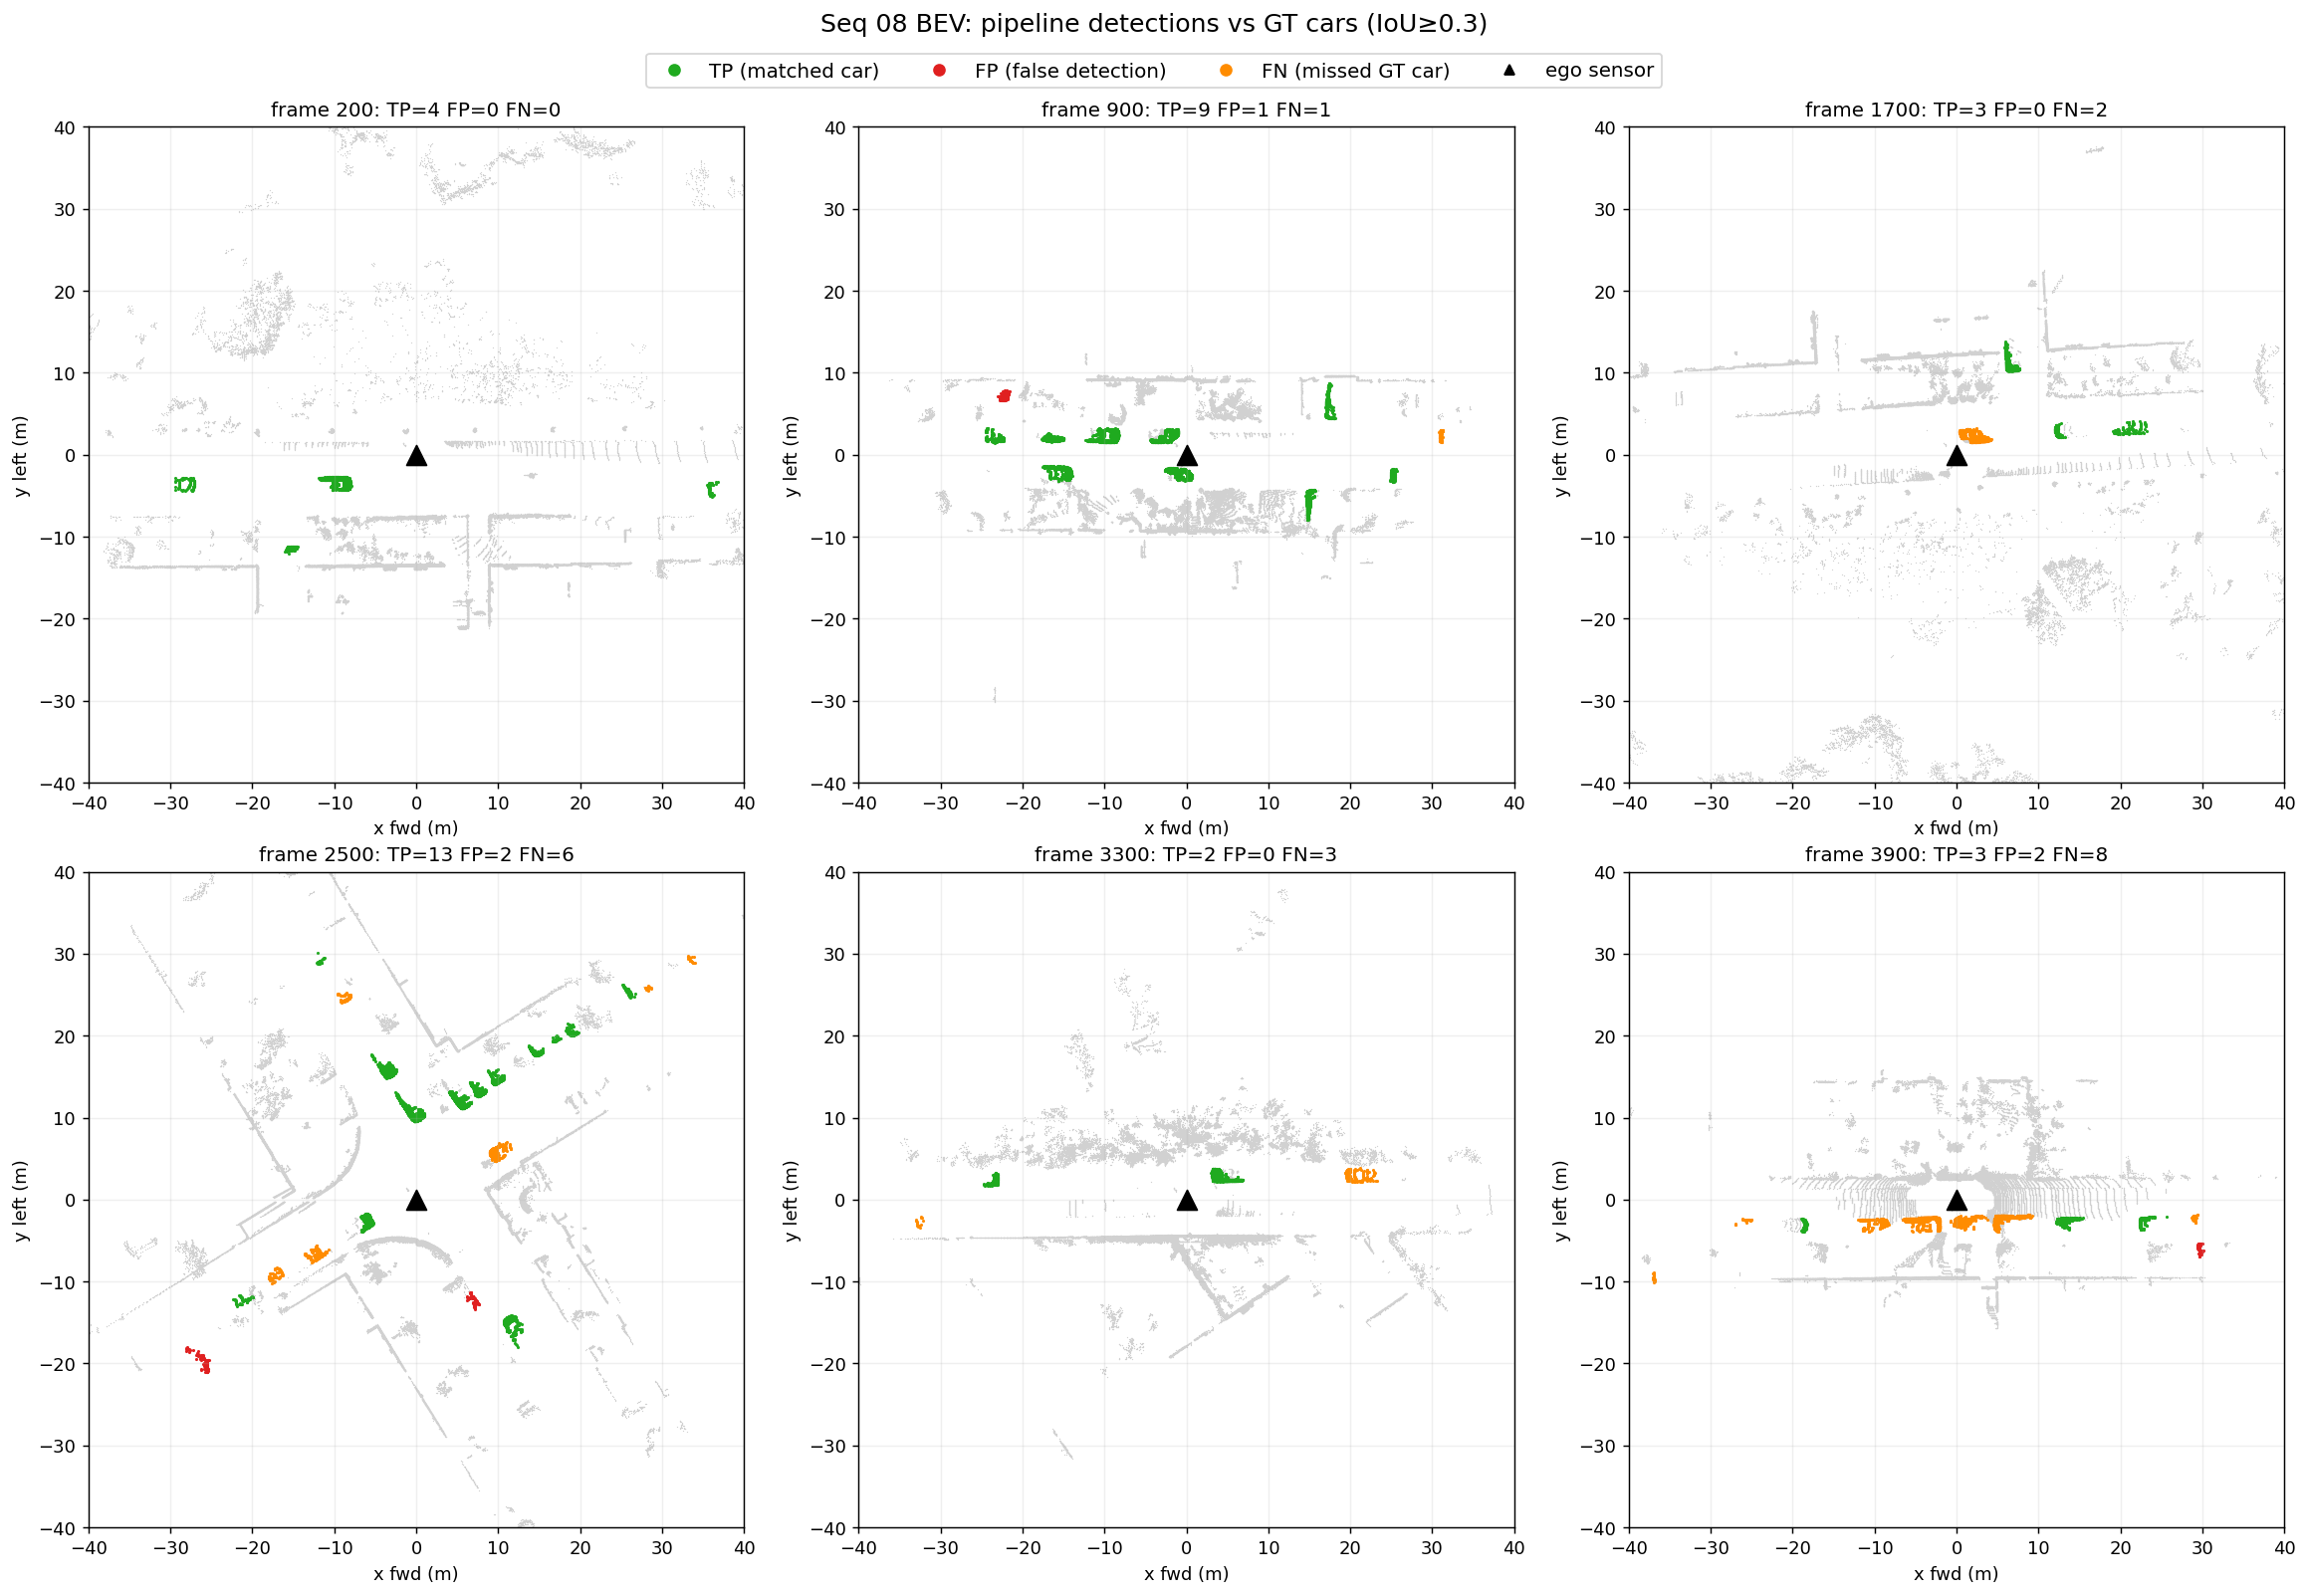
\includegraphics[width=\linewidth]{seq08_bev_detections.png}
  \caption[Bird's-eye view of detections on seq~08]{Bird's-eye view of detections on a representative sequence~08 frame.
    Detected car clusters (coloured) are overlaid on the ground-removed point
    cloud; ego is at the origin. Detections concentrate on true vehicles, with
    few spurious clusters, the precision-saturated behaviour reported in
    Table~\ref{tab:headline}.}
  \label{fig:bev-detections}
\end{figure}

\begin{figure}[htbp]
  \centering
  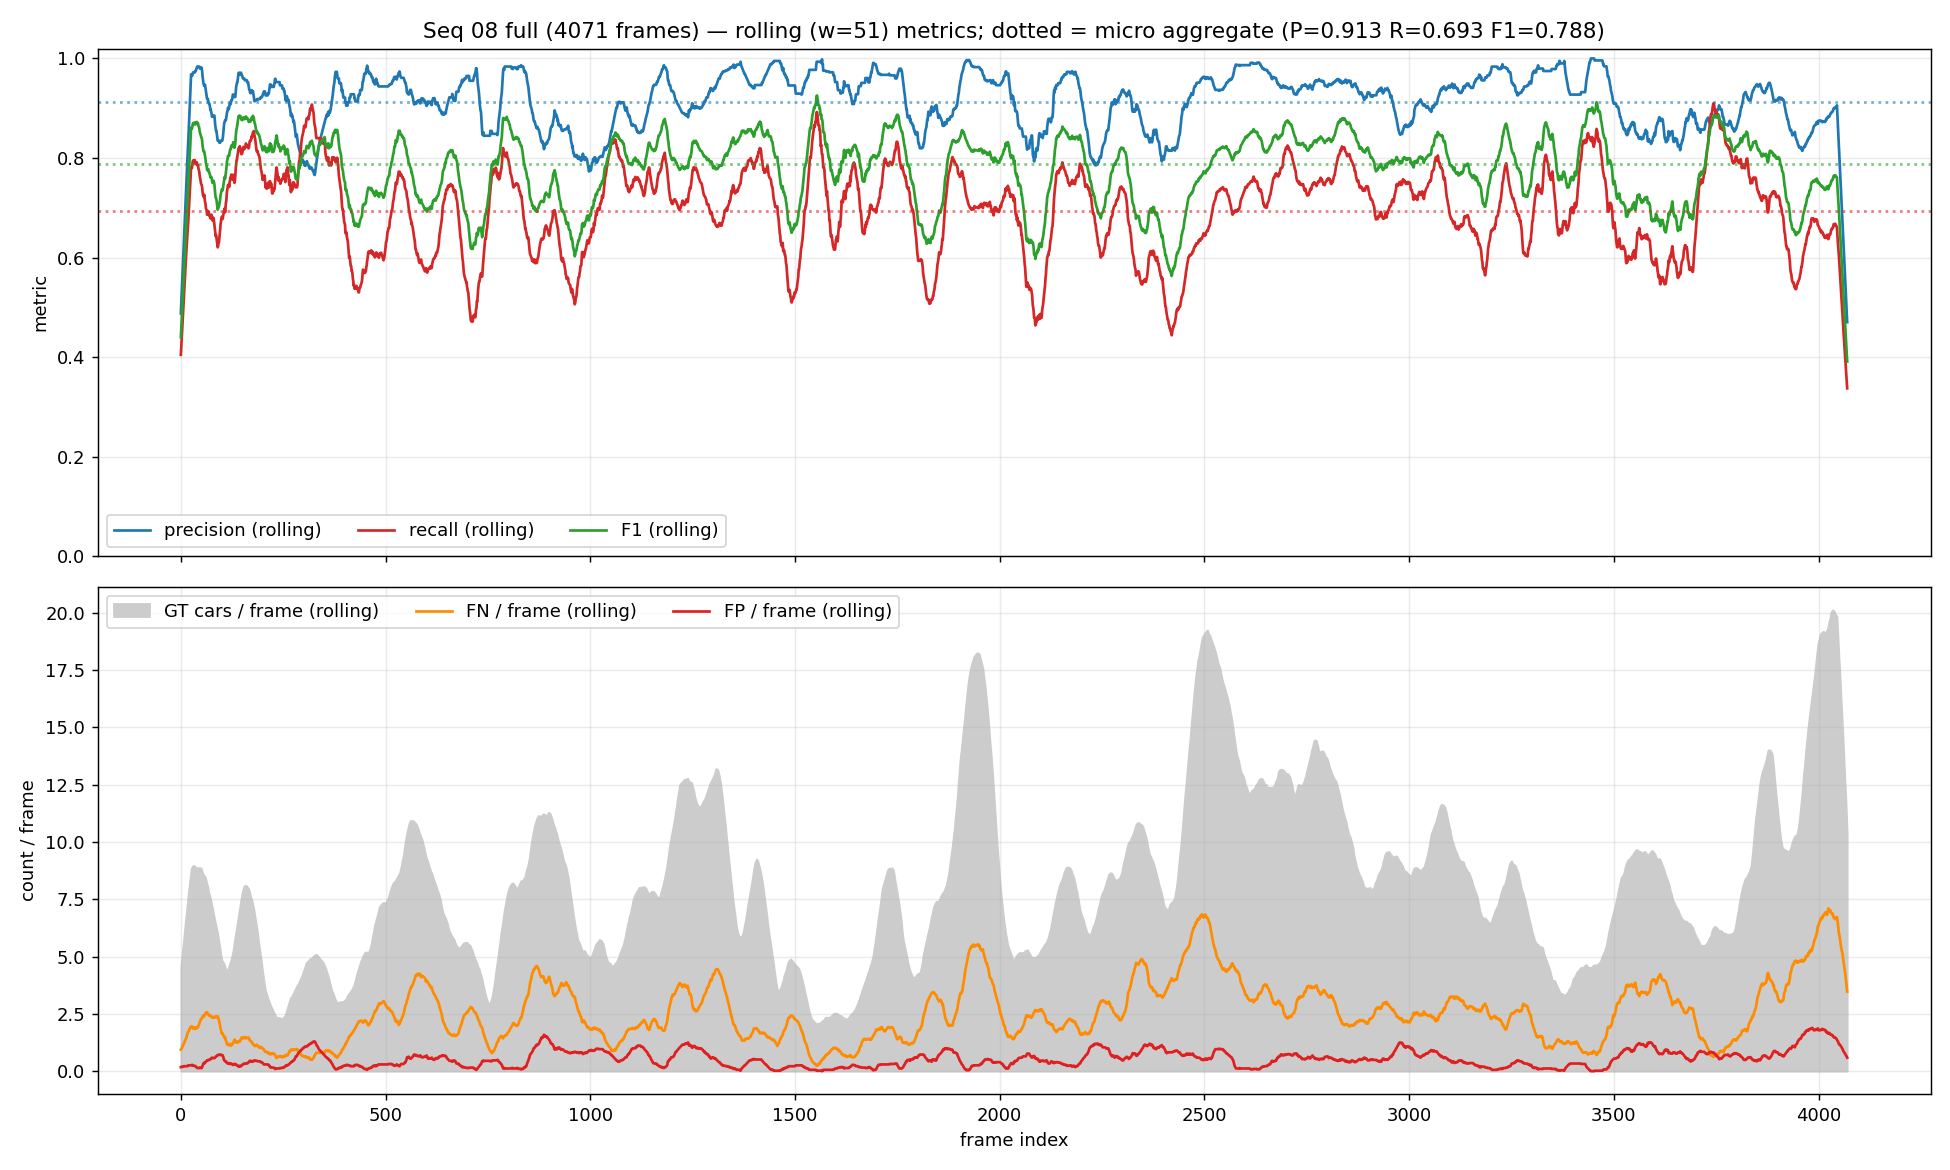
\includegraphics[width=\linewidth]{seq08_timeseries.png}
  \caption[Per-frame detection behaviour on seq~08]{Per-frame detection behaviour over sequence~08. False positives (lower
    trace) stay low and flat, under one per frame, regardless of scene
    content, while per-frame recall tends to fall in frames with more
    ground-truth cars. The structural recall limit is root-caused in Section~\ref{sec:recall-analysis}
    (HDBSCAN splitting).}
  \label{fig:timeseries}
\end{figure}

\subsection{Leave-One-Sequence-Out Cross-Validation}
\label{sec:eval-loso}

The operating point above is reported on sequence~08, which is also the sequence
the final classifier was historically selected on. To show that this selection
does not inflate the result, and to characterise the per-sequence recall spread
that a single reporting sequence cannot, we ran the LOSO protocol of
Section~\ref{sec:eval-sequences}: eleven folds, each training a classifier on ten
sequences and evaluating the full held-out eleventh, so every fold's classifier
is blind to the sequence it scores. Table~\ref{tab:loso} reports all eleven folds,
the pooled micro-average (counts summed across folds, comparable to the single
operating-point number), and the macro mean~$\pm$~standard deviation across folds.

\begin{table}[H]
  \centering
  \caption[Leave-one-sequence-out cross-validation]{Leave-one-sequence-out cross-validation over all eleven labelled
    sequences (full sequences, $\tau=0.3$, final configuration). Each fold's
    classifier trained on the other ten sequences and was never selected on the
    held-out one, so no row's classifier has seen the sequence it scores.
    ``Pooled'' sums TP/FP/FN across folds; the excl.-seq00 pool isolates the
    residual seq-00 classical-tuning familiarity (Section~\ref{sec:eval-sequences}).}
  \label{tab:loso}
  \setlength{\tabcolsep}{3pt}
  \footnotesize
  \begin{tabular}{lccccc}
    \toprule
    Held-out seq & Precision & Recall & $F_1$ & Mean IoU & TP / FP / FN \\
    \midrule
    00 (\num{4541} fr.) & 0.921 & 0.758 & 0.831 & 0.933 & \num{42583} / \num{3675} / \num{13607} \\
    01 (\num{1101} fr.) & 0.957 & 0.336 & 0.498 & 0.953 & \num{540} / \num{24} / \num{1066} \\
    02 (\num{4661} fr.) & 0.823 & 0.701 & 0.757 & 0.904 & \num{10941} / \num{2345} / \num{4663} \\
    03 (\num{801} fr.)  & 0.796 & 0.623 & 0.699 & 0.905 & \num{1528} / \num{391} / \num{925} \\
    04 (\num{271} fr.)  & 0.824 & 0.510 & 0.630 & 0.836 & \num{539} / \num{115} / \num{517} \\
    05 (\num{2761} fr.) & 0.880 & 0.725 & 0.795 & 0.910 & \num{10585} / \num{1448} / \num{4013} \\
    06 (\num{1101} fr.) & 0.873 & 0.637 & 0.737 & 0.906 & \num{6379} / \num{931} / \num{3632} \\
    07 (\num{1101} fr.) & 0.916 & 0.726 & 0.810 & 0.930 & \num{11089} / \num{1011} / \num{4179} \\
    08 (\num{4071} fr.) & 0.888 & 0.736 & 0.805 & 0.913 & \num{25715} / \num{3228} / \num{9207} \\
    09 (\num{1591} fr.) & 0.851 & 0.638 & 0.729 & 0.913 & \num{5072} / \num{888} / \num{2882} \\
    10 (\num{1201} fr.) & 0.745 & 0.557 & 0.638 & 0.872 & \num{1826} / \num{625} / \num{1450} \\
    \midrule
    \textbf{Pooled (all 11)} & \textbf{0.888} & \textbf{0.717} & \textbf{0.793} & \textbf{0.919} & \num{116797} / \num{14681} / \num{46141} \\
    Pooled (excl.\ seq~00)   & 0.871 & 0.695 & 0.773 & 0.912 & \num{74214} / \num{11006} / \num{32534} \\
    Macro mean $\pm$ std     & $0.861{\pm}0.059$ & $0.632{\pm}0.119$ & $0.721{\pm}0.095$ & $0.907{\pm}0.030$ &, \\
    \bottomrule
  \end{tabular}
\end{table}

Three things follow. First, model selection did not inflate the reported
recall. The fold-08 classifier, blind to sequence~08, reaches recall \num{0.736} against
the sequence-08 operating point's \num{0.732}, if anything marginally higher,
not lower, so the recall headline is not a product of having selected the
classifier on the reporting sequence. The model-selection optimism that does
exist is confined to precision and is small: fold-08 precision is \num{0.888}
versus the final \num{0.911} (an extra \num{715} false positives across
\num{4071} frames), exactly the two-point, precision-only exposure the stage
decomposition predicts (Section~\ref{sec:disc-eval-validity}). The two
sequence-08 rows are not two separate experiments but one classifier under
two checkpoint-selection rules: the final model and the fold-08 model share the
same architecture, the same ten training sequences (\numrange{00}{07},
\numrange{09}{10}), and the same from-scratch \num{15}-epoch regime, and differ
only in which epoch is frozen, the final model takes the epoch that scored
best on the sequence-08 validation set, the fold-08 model takes the last epoch and
never inspects sequence~08 at all. The \num{0.732}~$\rightarrow$~\num{0.736}
(recall) and \num{0.911}~$\rightarrow$~\num{0.888} (precision) deltas therefore
isolate the effect of that selection: selecting on sequence~08 bought about two
precision points and no recall. The isolation is not perfect, because
sequence~08 cannot serve as the fold's loss-monitoring split, the fold-08 model
trains on \SI{95}{\percent} of the final model's clusters (a \num{5}-percent
monitoring slice is set aside), but that confound removes training data from
the fold-08 model, which would depress its recall, not inflate it, so it only
strengthens the ``recall was not inflated'' reading. Second, the
pooled cross-validated operating point over all eleven sequences,
precision \num{0.888}, recall \num{0.717}, $F_1$~\num{0.793}, mean IoU
\num{0.919}, sits within roughly two points of the sequence-08 operating point
on every metric, so the reported numbers are representative of the labelled set
and not specific to sequence~08. Third, the per-sequence spread is now
explicit: recall ranges from \num{0.336} on sequence~01 (a sparse highway drive)
to \num{0.758} on sequence~00 (dense urban), with a macro mean of
\num{0.632}~$\pm$~\num{0.119}; precision is far steadier
(\num{0.861}~$\pm$~\num{0.059}). The gap between the pooled recall (\num{0.717})
and the macro mean (\num{0.632}) is driven by the smallest, sparsest sequences
(seq~01 and seq~04, the latter only \num{271} frames), which the count-weighted
pool down-weights and the unweighted mean does not; both figures are reported so
neither hides the spread. Finally, the residual seq-00 classical-tuning exposure
is bounded: dropping the seq-00 fold lowers pooled recall only from \num{0.717}
to \num{0.695} (a \num{0.022} delta), so the historical seq-00 pipeline tuning
does not drive the aggregate.

\subsection{Detection Accuracy Versus Range}
\label{sec:results-distance}

Recall is not uniform in range, and the way it varies is not the naive
``far~=~worse'' monotone one might expect. Table~\ref{tab:distance} stratifies
detection by the range of each cluster's centroid from the ego sensor, on a
stride-20 sample of sequence~08 under the frozen configuration.
Deviation: like the clustering benchmark, this table is
per-frame with the track filter off (striding breaks the tracker), so its
pooled recall (\num{0.671}) is a per-frame figure and does not restate the
track-filtered headline \num{0.732}; read the table as a range trend, not
as a re-derivation of the headline.

\begin{table}[H]
  \centering
  \caption[Detection stratified by range-to-ego on seq~08]{Detection stratified by range-to-ego on sequence~08 (stride-20 sample,
    frozen configuration, per-frame / track-filter-off). Recall is
    non-monotonic: it dips in the nearest bin, peaks at
    \SIrange{10}{20}{\metre}, then falls with range. The nearest-bin dip is
    over-segmentation, the far decline is sparsity. Mean IoU is
    over matched detections. Summing the two near bins recovers the
    \SIrange{0}{20}{\metre} figure ($R=\num{0.829}$) comparable to the earlier
    range analysis.}
  \label{tab:distance}
  \begin{tabular}{lccccc}
    \toprule
    Range (m) & Precision & Recall & $F_1$ & Mean IoU (matched) & TP / FP / FN \\
    \midrule
    0--10   & 0.899 & 0.787 & 0.839 & 0.902 & \num{311} / \num{35}  / \num{84}  \\
    10--20  & 0.869 & \textbf{0.862} & 0.866 & 0.926 & \num{432} / \num{65}  / \num{69}  \\
    20--40  & 0.799 & 0.550 & 0.652 & 0.934 & \num{401} / \num{101} / \num{328} \\
    40+     & 0.512 & 0.196 & 0.284 & 0.943 & \num{22}  / \num{21}  / \num{90}  \\
    \midrule
    Pooled  & 0.840 & 0.671 & 0.746 & 0.923 & \num{1166} / \num{222} / \num{571} \\
    \bottomrule
  \end{tabular}
\end{table}

The counter-intuitive result is the nearest-bin recall dip: recall at
\SIrange{0}{10}{\metre} (\num{0.787}) is lower than at
\SIrange{10}{20}{\metre} (\num{0.862}), even though near cars carry far more
points. This is not sparsity, it is over-segmentation. The split-rate analysis shows
that HDBSCAN splits the majority of the very-near cars (a split rate of
\SI{53.5}{\percent} at \SIrange{0}{10}{\metre}, falling to \SI{3.5}{\percent} past
\SI{40}{\metre}): a large, close car dissolves into several clusters,
none of which matches the whole instance, so it is counted as a miss. The nearest bin
also has the lowest mean IoU of matched detections (\num{0.902}),
consistent with fragments eroding the overlap even on the cars that do match. We
develop this splitting mechanism, and why post-hoc fragment-merging fails to
recover it, in Section~\ref{sec:recall-analysis}.

Beyond the peak the decline is ordinary sparsity: recall falls from \num{0.862}
at \SIrange{10}{20}{\metre} to \num{0.550} at \SIrange{20}{40}{\metre} and
\num{0.196} past \SI{40}{\metre}, as cars thin to too few surviving points to
cluster or to clear the \num{10}-point eligibility rule (Section~\ref{sec:eval-protocol}).
Mean IoU of matched detections rises with range
(\num{0.902}~$\rightarrow$~\num{0.943}): the far cars that are detected at all are
compact, single-cluster instances, so their overlap is clean even as their number
collapses. The earlier precision-only, seq-00, pre-promotion range analysis is superseded by this on-frozen-config sequence-08 table and is
retained only as a historical note.

\section{Runtime Evaluation}
\label{sec:results-runtime}

Table~\ref{tab:runtime} breaks the per-frame cost down by stage, measured over
the full sequence~08 under the final (promoted) configuration
(\num{4068} timed frames, RTX~3070~Ti / Ryzen~7~7800X3D;
per-stage figures from \texttt{timing\_seq08\_full\_n4068\_combined.json}). The breakdown shows where
the time goes: the two classical geometric stages, ground-plane RANSAC and,
above all, HDBSCAN clustering, dominate, together taking roughly
\SI{68}{\percent} of the frame; adding preprocessing and the geometric filter,
the classical CPU stages account for about \SI{94}{\percent}, leaving the single
learned component, the classifier, at only $\sim$\SI{5.4}{\percent} (the
centroid/Hungarian tracker is a classical assignment step, not learned). The
classifier is \SI{33.7}{\milli\second} for the $\sim$\num{45} clusters in a frame
($\sim$\SI{0.75}{\milli\second} each) and the tracker is negligible.

\begin{table}[H]
  \centering
  \caption[Per-frame runtime by stage on seq~08]{Per-frame runtime by stage on the full sequence~08 under the final
    (promoted) configuration (\num{4068} timed frames; mean ms).
    Clustering alone is nearly \SI{60}{\percent} of the frame. The total is
    $\approx\SI{623.5}{\milli\second}$ ($\approx$\num{1.6}~fps) on this full run;
    a stride-20 sample of the same configuration estimates
    $\approx\SI{650.6}{\milli\second}$ (the two agree to within the sampling
    variation of the expensive stages). The pre-optimisation configuration
    totalled \SI{921.3}{\milli\second}. Percentages are of the
    \SI{623.5}{\milli\second} total.}
  \label{tab:runtime}
  \begin{tabular}{lcc}
    \toprule
    Stage & Mean (ms) & Share \\
    \midrule
    Data load                       & 0.7   & 0.1\% \\
    Preprocessing (z-filter, denoise, voxel) & 125.9 & 20.2\% \\
    Ground removal (RANSAC)         & 56.2  & 9.0\% \\
    Clustering (HDBSCAN)            & 370.4 & 59.4\% \\
    Geometric filter                & 36.2  & 5.8\% \\
    Classification                  & 33.7  & 5.4\% \\
    Tracking                        & 0.3   & 0.1\% \\
    \midrule
    Total                           & 623.5 & 100\% ($\approx$1.6 fps) \\
    \bottomrule
  \end{tabular}
\end{table}

The promoted configuration is itself the product of a runtime optimisation that
targeted the dominant classical stages directly: reducing the
RANSAC iteration count and coarsening the clustering voxel to \SI{0.10}{\metre}
cut the per-frame total by roughly a third, from a pre-optimisation
\SI{921.3}{\milli\second} to \SI{623.5}{\milli\second} on the full sequence
(\SI{650.6}{\milli\second} on the stride-20 sample), and the coarser voxel also
improved detection, it is the promoted configuration used throughout
this chapter. A sub-\SI{400}{\milli\second} target was shown to be unreachable
through the authorised optimisation tiers, the post-ground object cloud is
intrinsically sparse, so coarser voxelisation compresses it little and the Python
HDBSCAN retains a floor of $\sim$\SI{185}{\milli\second}, and the achieved
operating point was accepted, real-time operation being out of scope (user
decision, \num{2026}-07-23). Point-completion, when it runs, adds
$\sim$\SI{13}{\milli\second} per completed car on top of detection and is not part
of the detection budget above.


%% ===== merged from sec_5_recall_bottleneck.tex ===== %%

% The Recall Bottleneck (folds under Chapter 4 as a section, not a chapter of its own).
% Root-causes the recall shortfall established earlier in the chapter and reports the
% failed repair strategies as a negative-results contribution. Sub-tables are
% referenced by section + Finding number rather than hard-coded table number, to stay
% robust to renumbering.
%
% Honesty-phrasing rules applied (personal_agenda P1):
%   - recall denominator restated / cross-referenced (>=10 surviving points, Sec 4.1)
%   - "mean IoU" always qualified as "of matched detections"
%   - negative results (#21/#24, temporal aggregation) reported AS FINDINGS, not
%     apologised for
%   - the retracted "~0.74 hard limit" is corrected explicitly (#24 Correction / #34)
%   - two measurement eras kept separate: the pre-promotion seq-00 repair search
%     (baseline F1 0.844; #21/#24/temporal) vs the promoted-config seq-08 fix (#34)
%   - every number traces to a finding / session log artifact (cited Finding~\#NN /
%     session_history.md)
%
\section{Completion Results}
\label{sec:results-completion}
\label{sec:completion-results}

The completion stage is evaluated on the two fronts the problem allows. On
synthetic shapes a complete ground truth exists, so the network can be scored
directly with Chamfer distance and F-score; this establishes that the network works in
distribution (Section~\ref{sec:results-synthetic}). On real LiDAR no complete
ground-truth shape exists (Section~\ref{sec:bg-completion}), so the completion is judged
two ways that need no self-made reference: an independent shape classifier tests whether
the completed real clouds read as cars (Section~\ref{sec:results-plausibility}), the
favorable real-data signal; and the established reference-free fidelity metrics are
reported with the caveat that they reward under-completion
(Section~\ref{sec:results-fidelity}). The scope of the resulting claim is stated plainly in
Section~\ref{sec:results-completion-scope}.

\subsection{Synthetic Fidelity: The Network in Distribution}
\label{sec:results-synthetic}

Trained on the KITTI-like synthetic partials of Section~\ref{sec:completion-kittilike}
(input \num{256} points, target the dense mesh sample), the completion network
(\texttt{pcn\_kitti\_best.pth}) reaches a best validation Chamfer loss of \num{0.1246}. On
a held-out synthetic set, where the complete CAD shape is the ground truth, it produces
clean cars rather than blobs: Chamfer distance \SI{0.16}{\meter} and
F-score@\SI{0.1}{\meter} \num{0.76}. These are established metrics against an established
ground truth (ShapeNet), and they confirm the network has learned the partial-to-complete
mapping in distribution. They say nothing on their own about real LiDAR, which is what the
next two subsections address.

\subsection{Real-Data Plausibility: An Independent Classifier}
\label{sec:results-plausibility}

On real cars there is no complete shape to score against, so we adopt the plausibility
protocol of Chen et al.~\cite{chen2020unpaired}: an independent shape classifier,
trained on complete-shape data disjoint from the completion network's training set, judges
whether each completed cloud reads as a car. The judge is a PointNet++ (single-scale
grouping) trained from scratch on ModelNet40, whose CAD models are drawn from a different
repository than the ShapeNet cars PCN was trained on, so a car accepted by the judge is not
an artefact of shared training data. Chen et al.\ use a ModelNet40-trained judge for exactly
this reason. The judge reaches \num{0.9214} test accuracy on ModelNet40 (above a
pre-registered \num{0.88} usability gate) and is trained without rotation augmentation, so
it is orientation-sensitive; every cloud is therefore harmonised into the judge's canonical
frame (width, up, length), resampled to \num{1024} points and unit-sphere normalised, before
scoring. The experiment and its hypotheses were pre-registered before any scoring run.

We score \num{2822} completed car tracks across all eleven labelled sequences, each paired
with its own raw single-frame partial, and report the car-acceptance rate (the fraction the
judge labels car) and the mean car-probability. As a shape-quality upper bound we also score
\num{140} static-accumulation clouds: dense multi-frame accumulations of well-observed
static cars, which are both dense and correctly shaped, the ceiling a completion could aspire
to. Table~\ref{tab:plausibility} reports the three arms.

\begin{table}[H]
  \centering
  \caption[Independent-classifier plausibility of completed cars]{Independent-classifier
    plausibility on real LiDAR cars (pooled over all eleven labelled sequences,
    $N=\num{2822}$ paired raw/completed tracks; the static-accumulation ceiling is a
    separate $N=\num{140}$ set of dense, correctly-shaped cars). Acceptance is the judge's
    car argmax rate; car-probability is its mean car posterior. The raw$\to$completed
    contrast is paired; the completed$\to$ceiling contrast is across different car
    populations.}
  \label{tab:plausibility}
  \begin{tabular}{lcc}
    \toprule
    Arm & Acceptance $\uparrow$ & Mean car-prob $\uparrow$ \\
    \midrule
    Raw partial            & 0.253          & 0.219 \\
    \textbf{Completed}     & \textbf{0.785} & \textbf{0.745} \\
    Static-accumulation ceiling & 0.807     & 0.728 \\
    \bottomrule
  \end{tabular}
\end{table}

Completion raises car-acceptance from \num{0.253} on the raw partials to \num{0.785}, and
mean car-probability from \num{0.219} to \num{0.745}. The paired gain is decisive: on a
McNemar test of the paired argmax decisions, completion flips \num{1615} rejected partials
to accepted against only \num{115} in the reverse direction ($p\approx0$), and the paired
car-probability improvement is significant on a Wilcoxon signed-rank test ($p\approx0$).
This is the primary favorable real-data completion result: an external judge, with no stake
in the completion network's training data, reads the completed clouds as cars far more often
than the partials it started from.

\paragraph{Completion reaches the shape-quality ceiling:} The raw$\to$completed gain could
in principle be a density effect: the completion is denser than the partial, and the judge
might reward density alone. The static-accumulation ceiling controls for this, because it is
both dense and correctly shaped. The completed clouds reach it: on the static
subset ($N=\num{2220}$) the completed mean car-probability is \num{0.730}, statistically at
the ceiling's \num{0.728} (Mann-Whitney $p=\num{6.8e-7}$ reflects distribution shape at
large $N$, with the completed central tendency at or above the ceiling), and completed
acceptance \num{0.770} recovers about \num{96}\% of the raw$\to$ceiling acceptance gap. A
completion that merely produced denser blobs would sit well below a ceiling built from
correctly-shaped cars; that it reaches the ceiling is evidence the completed shapes are
genuinely car-like, not just dense.

\begin{figure}[H]
  \centering
  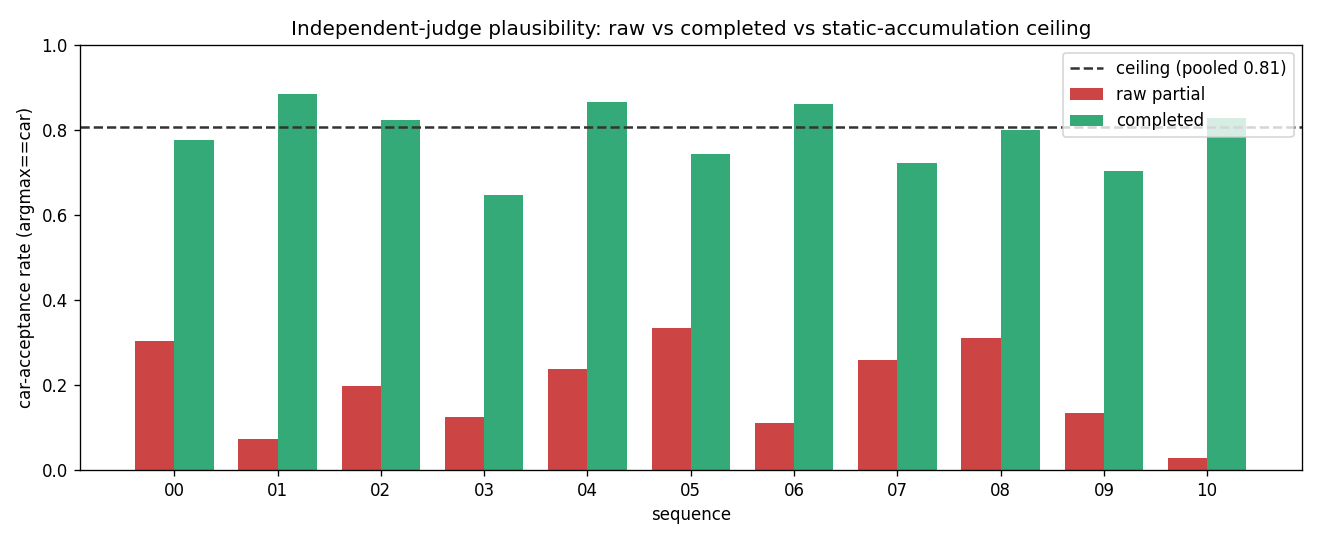
\includegraphics[width=\linewidth]{plausibility_acceptance.png}
  \caption[Plausibility by sequence]{Car-acceptance of the independent judge, per sequence:
    raw single-frame partial (red) against the PCN completion (green), with the pooled
    static-accumulation ceiling (dashed). Completion lifts acceptance several-fold on every
    one of the eleven labelled sequences and sits at or near the ceiling throughout;
    sequence~08, on which the completion constants were tuned, is not an outlier, so the
    result is not an artefact of tuning.}
  \label{fig:plausibility}
\end{figure}

\paragraph{The gain holds on every sequence:} The completion constants were developed on
sequence~08, so a fair test is whether the plausibility gain appears on sequences that took
no part in that development. Figure~\ref{fig:plausibility} and Table~\ref{tab:plausibility-seq}
show it does: completed acceptance ranges from \num{0.646} to \num{0.885} across the eleven
sequences, several times the raw-partial rate on each, and sequence~08 (\num{0.311}
$\to$~\num{0.799}) is unremarkable among them. The completion network was trained only on
synthetic data and never saw any real sequence, so this consistency is a direct
generalisation result.

\begin{table}[H]
  \centering
  \caption[Plausibility acceptance by sequence]{Car-acceptance by sequence, raw partial vs.\
    completed, over all eleven labelled sequences ($N$ = paired tracks per sequence).}
  \label{tab:plausibility-seq}
  \small
  \setlength{\tabcolsep}{4.5pt}
  \begin{tabular}{lccccccccccc}
    \toprule
    Seq & 00 & 01 & 02 & 03 & 04 & 05 & 06 & 07 & 08 & 09 & 10 \\
    \midrule
    $N$ & 926 & 96 & 329 & 48 & 59 & 258 & 164 & 213 & 518 & 141 & 70 \\
    Raw & 0.30 & 0.07 & 0.20 & 0.13 & 0.24 & 0.33 & 0.11 & 0.26 & 0.31 & 0.13 & 0.03 \\
    Compl.\ & 0.78 & 0.89 & 0.82 & 0.65 & 0.86 & 0.74 & 0.86 & 0.72 & 0.80 & 0.70 & 0.83 \\
    \bottomrule
  \end{tabular}
\end{table}

\paragraph{Moving cars complete as plausibly as static ones:}
\label{sec:results-movers}
Because completion runs on a single reference frame's cluster rather than on accumulated
points, there is no motion smear in its input, so motion is not expected to matter. Labelling
each track static or moving by the net displacement of its centroid confirms it: the moving
subset ($N=\num{602}$) reaches completed acceptance \num{0.837} and car-probability
\num{0.801}, if anything slightly above the static subset. The static-only ceiling comparison
above therefore does not hide a mover failure mode.

\paragraph{Heading ambiguity is not a confound:} The harmonisation fixes each cloud's up axis
and length axis but leaves front-versus-back ambiguous (the footprint fit does not resolve
heading sign). Re-scoring every completed cloud with an added \SI{180}{\degree} heading flip
changes acceptance by only \num{0.009}, so the residual heading ambiguity does not affect the
result.

\subsection{Reference-Free Fidelity and Its Caveat}
\label{sec:results-fidelity}

The field's established reference-free metrics score a completion by how closely it reproduces
its own observed input: the unidirectional Chamfer and Hausdorff distances (UCD, UHD;
Section~\ref{sec:th-distances}), applied to real KITTI cars by Chen et
al.~\cite{chen2020unpaired} and P2C~\cite{cui2023p2c}. Computed on the seq-08 cars
(input\,$\to$\,cloud direction, per-car medians), they behave exactly as their definition
dictates (Table~\ref{tab:fidelity}): the raw partial is a trivial optimum at \num{0}, because
it is its own input, while the completion is scored worst, penalised for every point it
adds beyond the observed side.

\begin{table}[H]
  \centering
  \caption[Reference-free fidelity metrics]{Reference-free fidelity on seq-08 cars
    (\num{39} cars, per-car medians, input\,$\to$\,cloud direction; lower is ``better'' in the
    sense of reproducing the observed input). The raw partial is the trivial optimum and the
    completion scores worst, the metrics reward under-completion, which is why they cannot
    on their own credit a completion and why the plausibility signal above is the load-bearing
    real-data evidence.}
  \label{tab:fidelity}
  \begin{tabular}{lccc}
    \toprule
    Cloud & UCD (m) $\downarrow$ & UHD$_{\max}$ (m) $\downarrow$ & UHD$_{p95}$ (m) $\downarrow$ \\
    \midrule
    Raw partial        & 0.000 & 0.000 & 0.000 \\
    Mirrored           & 0.000 & 0.000 & 0.000 \\
    \textbf{Completed} & 0.090 & 0.286 & 0.183 \\
    \bottomrule
  \end{tabular}
\end{table}

This is not a negative result about the completion; it is a property of the metrics. An
input-fidelity measure is minimised by the cloud that adds nothing, so it structurally cannot
reward recovering unobserved surface. This is precisely why the unpaired-completion literature
pairs UCD/UHD with a separate plausibility term~\cite{chen2020unpaired}, and why this thesis
reports fidelity honestly here but rests its favorable real-data claim on the plausibility of
Section~\ref{sec:results-plausibility}.

\subsection{Scope of the Completion Claim}
\label{sec:results-completion-scope}

The completion evidence is deliberately scoped. The network works in distribution on
synthetic shapes (Chamfer \SI{0.16}{\meter}, F@\SI{0.1}{\meter} \num{0.76}), but synthetic
performance is not a real-data claim. On real LiDAR the favorable evidence is the
independent-classifier plausibility: completion lifts car-acceptance from \num{0.253} to
\num{0.785}, reaching the static-accumulation shape ceiling, consistently across all eleven
sequences and for moving as well as static cars. The reference-free fidelity metrics do not
credit the completion, and are reported as such rather than omitted. The claim the thesis
makes is therefore this and no more: on real automotive LiDAR, learned completion produces
shapes an independent classifier accepts as cars far more often than the raw partials, and as
often as dense correctly-shaped references, while established fidelity metrics, which reward
reproducing the input, do not credit it. A remaining limitation of the production path is the
per-car length estimate's fixed-prior fallback on tracks with fewer than five gate-passed
frames (Section~\ref{sec:completion-length}); on the seq-08 output this fallback is used by a
non-trivial fraction of tracks and is revisited in the discussion.

\section{Ablation Studies}
\label{sec:results-ablations}

This section decomposes both halves of the system into the contribution of each
component, in two groups: detection ablations
(Section~\ref{sec:abl-detection}) and completion ablations
(Section~\ref{sec:abl-completion}). Every ablation is produced under the frozen
protocol of Section~\ref{sec:eval-protocol} unless a deviation is stated explicitly.

\subsection{Detection Ablations}
\label{sec:abl-detection}

\paragraph{Stage decomposition (classifier and track filter):}
\label{sec:ablation-stage}

Table~\ref{tab:ablation-stage} isolates the two filtering stages that sit on top
of geometric clustering. The geometric-only row uses clustering plus the
geometric size/shape filters with no learned classifier and no
track filter (like-for-like under the promoted
configuration); the full row is the headline.

\begin{table}[H]
  \centering
  \caption[Stage ablation on seq~08]{Stage ablation on the full sequence~08 (frozen configuration). Rows
    add one filtering stage at a time on top of geometric clustering. The
    per-frame classifier is the precision mechanism (it removes $\sim$\num{104000}
    junk clusters) but is conservative on borderline cars (recall drops); the
    offline track filter then recovers recall by temporal voting while raising
    precision further. Mean IoU is over matched detections only. Geometric-only
    and the middle row are per-frame (no track filter); the full row uses the
    offline track filter.}
  \label{tab:ablation-stage}
  \setlength{\tabcolsep}{5pt}
  \begin{tabular}{lccccc}
    \toprule
    Configuration & Precision & Recall & $F_1$ & Mean IoU & TP / FP / FN \\
    \midrule
    Geometric only                & 0.199 & 0.773 & 0.316 & 0.907 & \num{27002} / \num{108831} / \num{7920} \\
    \;+\,classifier              & 0.846 & 0.676 & 0.751 & 0.922 & \num{23600} / \num{4303} / \num{11322} \\
    \;+\,classifier, track filter & 0.911 & 0.732 & 0.812 & 0.913 & \num{25568} / \num{2513} / \num{9354} \\
    \bottomrule
  \end{tabular}
\end{table}

The decomposition tells a two-step story. The classifier
is the precision mechanism: geometric clustering under the promoted coarse-voxel
setting emits many mostly-junk clusters (precision \num{0.199}), and the per-frame
classifier removes about \num{104000} of them across the sequence
(FP \num{108831}~$\rightarrow$~\num{4303}), lifting precision from \num{0.199} to
\num{0.846}. It pays for this with recall, being conservative, it discards
borderline true clusters too, so recall falls from \num{0.773} to \num{0.676}.
The track filter then recovers that recall while improving precision
again: linking detections across frames and accepting only consistent tracks
lifts precision to \num{0.911} and recall to \num{0.732} (TP
\num{23600}~$\rightarrow$~\num{25568}), because a car seen across many frames is
kept even where a single frame classified it as unknown, while transient
false positives fail the track-length test. The net of both stages is still a
recall trade, geometric-only recall (\num{0.773}) exceeds the full-pipeline
recall (\num{0.732}), roughly \num{1400} true positives forgone for the
$\sim$\num{106000}-false-positive removal, but that trade runs through a
recall dip and a partial recovery, not a simple monotone loss. We report it
rather than hiding it: the system is deliberately tuned for precision, and the
recall it forgoes here is small next to the recall it never had (Section~\ref{sec:recall-analysis}). The
pre-promotion geometric-only figure ($F_1$~\num{0.305}) is
superseded by this like-for-like \num{0.316} and kept only as a historical
record.

\paragraph{Redundancy of synthetic pretraining (Stage~A ablation):}
\label{sec:ablation-stagea}

The classifier ships as a binary car/not-car network trained from scratch
on mined real clusters (Stage~B). A natural alternative is a two-stage
recipe in which a synthetic-ShapeNet Stage~A pretraining seeds Stage~B; we tested
whether that pretraining is necessary and found it is not, a negative result we
report as a finding, because it changes the recommended recipe.

At the classifier level, on the sequence~08 validation clusters, the from-scratch
network matches the pretrained one: macro $F_1$ \num{0.9285} from scratch versus
\num{0.9225} pretrained (the two are within run-to-run noise, with
scratch marginally ahead). At the pipeline level the two checkpoints are
identical in $F_1$ to three decimals on the full sequence~08. We therefore
drop Stage~A from the production pipeline and keep it as ablation material.

The reason the synthetic prior is redundant, and cannot simply be added for
safety, is a total, symmetric domain gap between synthetic and real point
clusters. Table~\ref{tab:cross-domain} gives the cross-domain
transfer matrix: a model trained on one domain and evaluated on the other scores
a car-class $F_1$ of \num{0.000} in both off-diagonal directions, and
fine-tuning on real data erases whatever the synthetic pretraining had learned.
Given \num{420000} real training clusters, the real data does essentially all the
work; the synthetic prior neither helps nor, once fine-tuned, survives.

\begin{table}[H]
  \centering
  \caption[Cross-domain classifier transfer]{Cross-domain classifier transfer (car-class $F_1$). Each
    model is trained on one domain and evaluated on the other's validation set;
    diagonal cells (italic) are in-domain, for scale. Both off-diagonal cells
    collapse to \num{0.000}, against strong in-domain performance
    (\num{0.999}, \num{0.885}), so synthetic and real clusters are mutually
    out-of-distribution and synthetic pretraining transfers nothing to real
    inference.}
  \label{tab:cross-domain}
  \begin{tabular}{lcc}
    \toprule
    & \multicolumn{2}{c}{Evaluated on} \\
    \cmidrule(lr){2-3}
    Trained on & Synthetic & Real \\
    \midrule
    Synthetic (Stage~A) & 0.999 & 0.000 \\
    Real (Stage~B)      & 0.000        & 0.885 \\
    \bottomrule
  \end{tabular}
\end{table}

\paragraph{Cost and benefit of HDBSCAN clustering:}
\label{sec:ablation-clustering}

The clustering stage is HDBSCAN. Because it is by far the most expensive stage
(Section~\ref{sec:results-runtime}), we benchmarked it against two cheaper
density/connectivity clusterers, DBSCAN and Euclidean-tolerance clustering,
at the same voxel resolution and under an identical pipeline
(Table~\ref{tab:clustering}). Deviation: this benchmark is
per-frame with the track filter off, because it strides across the
sequence and the tracker requires contiguous frames; the numbers are therefore
comparable to each other but not to the track-filtered headline.

\begin{table}[H]
  \centering
  \caption[Clustering-method benchmark]{Clustering-method benchmark at fixed voxel resolution
    ($\SI{0.10}{\metre}$), identical pipeline, per-frame / track-filter-off. HDBSCAN wins $F_1$ on both sequences, entirely through
    recall; precision is essentially method-independent. The alternatives are
    4--6$\times$ faster. Mean IoU is over matched detections; the timing column is
    the mean per-frame clustering time.}
  \label{tab:clustering}
  \begin{tabular}{llccccc}
    \toprule
    Seq & Method & Precision & Recall & $F_1$ & Mean IoU & Clustering (mean ms) \\
    \midrule
    \multirow{3}{*}{00}
      & HDBSCAN   & 0.972 & \textbf{0.731} & \textbf{0.835} & 0.968 & 306 \\
      & DBSCAN    & 0.975 & 0.637 & 0.771 & 0.964 & 54 \\
      & Euclidean & 0.979 & 0.636 & 0.771 & 0.982 & 76 \\
    \midrule
    \multirow{3}{*}{08}
      & HDBSCAN   & 0.840 & \textbf{0.671} & \textbf{0.746} & 0.923 & 320 \\
      & DBSCAN    & 0.870 & 0.565 & 0.685 & 0.927 & 57 \\
      & Euclidean & 0.869 & 0.576 & 0.693 & 0.950 & 75 \\
    \bottomrule
  \end{tabular}
\end{table}

The gap is entirely a recall gap, precision is within \num{0.030} across all
methods on either sequence, while HDBSCAN's recall exceeds the alternatives by
\numrange{9}{11} points. An $\varepsilon$-sweep confirms no fixed radius closes
it: the best fixed-radius setting (Euclidean at $\varepsilon=\SI{0.4}{\metre}$)
reaches $F_1$ \num{0.800} on sequence~00, still short of HDBSCAN's \num{0.835}.
HDBSCAN's variable-density criterion recovers cars that a single radius cannot,
which is exactly the recall margin that matters here. We therefore
adopt nothing from the benchmark and keep HDBSCAN in production, paying
its runtime cost knowingly; DBSCAN and Euclidean remain available as
command-line options for reproduction.

\subsection{Completion Ablations}
\label{sec:abl-completion}

These ablations isolate the effect of each completion-pipeline choice; they vary one
component of the completion path (Section~\ref{ch:completion-method}) and re-run the
completion, with the completion network itself unchanged.

\paragraph{Inference normalisation:} PCN is trained in a canonical car frame, so a real
partial must be mapped into that frame before completion
(Section~\ref{sec:completion-normalisation}). The importance of this step is the
semantics-map lesson of Section~\ref{sec:completion-inferencebug} made concrete: with the
canonical-frame normalisation, the completed clouds are recognisably car-shaped and
correctly oriented; with a naive alternative, aligning the partial to a 3D PCA frame and
normalising by its own centroid and radius, the same checkpoint produces mis-oriented,
mis-scaled blobs, because the 3D PCA picks an arbitrary principal axis rather than gravity.
The blob-versus-car difference is entirely a normalisation effect, not a network one, since
the checkpoint is identical.

\paragraph{Input-quality gate:} The L-shape gate decides whether a detected car reaches
completion as a clean single-object cluster (Section~\ref{sec:completion-lshape}). It
rejects HDBSCAN fragments and merges, which would otherwise feed the completion network an
input that is not one whole car and complete into an implausible shape. On seq~08 every
implausible completion originated from a fragment or merge input, so the gate is what keeps
the production completions clean; it carries a measured cost, dropping a fraction of
otherwise-usable cars as false rejections, which is stated as a limitation rather than
hidden.

\paragraph{Length geometry:} A partial truncated at the occluded far end completes short,
so the completion tends to under-extend length (Section~\ref{sec:completion-length}). The
production path corrects this with a per-car length estimate rather than a single fixed
prior, because a population-median prior over-extends genuinely compact cars while
under-extending long ones. The per-car estimate is the frozen production choice; a residual
far-end under-extension on the longest cars remains, characterised rather than eliminated,
and is carried to the discussion.

\paragraph{Completion architecture (PCN vs.\ PoinTr):} Swapping the completion network
holds the rest of the pipeline fixed. On held-out synthetic cars PoinTr's edge over PCN is
small (Chamfer \SI{0.161}{}$\to$\SI{0.153}{\meter}), a difference too small to justify the
heavier model, and the residual real-data gap is a centroid-estimation limit that is
architecture-independent. PCN is therefore kept off the shelf; the completion result is set
by input quality and geometry, not by the choice of network.

\section{Result Analysis and Error Analysis}
\label{sec:recall-analysis}

The detection operating point above established two facts: the pipeline is
precision-saturated (false positives are low and flat, about \num{0.6} per frame),
and it is recall-limited, missing roughly one car in four
($R=\num{0.732}$ on sequence~08). This section explains why the recall is
limited, and it also underpins the completion results reported earlier
(Section~\ref{sec:results-completion}): the same clustering step that caps recall
is the one that decides whether a detected car reaches completion as a clean
single-object cluster. We show that the shortfall is
a clustering failure rather than a classification failure
(Section~\ref{sec:recall-diagnosis}), root-cause it to HDBSCAN splitting large,
close cars into fragments (Section~\ref{sec:split-analysis}), report a search of
repair strategies that all fail to generalise (Section~\ref{sec:repairs}), and
describe the one intervention that did help, coarsening the clustering
resolution, which forces a correction of an earlier, overstated ``hard
ceiling'' claim (Section~\ref{sec:resolution-fix}). The negative results are
reported as findings, not apologised for: mapping which repairs fail, and why, is
itself a finding worth reporting, and it is what justifies the residual limitation carried to
Chapter~\ref{ch:conclusion}. Unless stated otherwise, the recall denominator
throughout is the one defined in Section~\ref{sec:eval-protocol}, ground-truth
car instances with at least \num{10} points surviving preprocessing.

\subsection{The Shortfall as a Clustering Failure}
\label{sec:recall-diagnosis}

The recall ceiling is upstream of the learned classifier. The stage decomposition
of Section~\ref{sec:results-ablations} makes this direct: geometric clustering with the
size/shape filters but no learned classifier and no track filter
already reaches recall \num{0.773}, which is higher than the full pipeline's
\num{0.732}. Every learned stage that follows can only hold or reduce that recall:
the classifier discards clusters, and the centroid tracker only re-labels and
filters clusters that geometric clustering has already produced, it emits a
detection in a frame only where a cluster exists in that frame, and never
interpolates a detection across a gap, so neither stage can invent a detection where clustering
found nothing. Across the full sequence the two stages together trade roughly
\num{1400} true positives (\num{27002} geometric-only versus \num{25568} full) for the removal of $\sim$\num{106000} false positives; this is a
distinct trade from the $+\num{756}$ true positives that the resolution change of
Section~\ref{sec:resolution-fix} later recovers. Whatever caps recall is therefore
already present in the clusters that geometric clustering produces, before the
classifier sees them.

The geometric filters are not the cap either. Ablation of the
size/shape gates across the full sequence~08 shows that of the
\num{903901} HDBSCAN clusters, \num{127654} (\SI{14.1}{\percent})
pass the filters, and \num{27718} of the rejected clusters overlap a ground-truth
car, dominated by \texttt{min\_volume} (\SI{73.9}{\percent} of the GT-matching
rejections) and \texttt{min\_points} (\SI{12.7}{\percent}). The dominant gates are
\texttt{min\_volume} and \texttt{min\_points}, the two that reject small
clusters. This is consistent with the rejected clusters being the smaller
sub-fragments of cars that HDBSCAN has already split (the dominant fragment passing
while the splinters fail the size gates), which the split analysis of
Section~\ref{sec:split-analysis} then confirms is the prevailing failure mode. We
state this as an inference rather than a direct measurement: the ablation records
only that a rejected cluster overlaps some ground-truth car,
not whether that same car also retains a
surviving cluster, so it establishes that the rejections are dominated by small
fragments, not that every one belongs to an otherwise-detected car. Either way the
diagnosis points one stage further upstream, at the clustering itself.

\subsection{Root Cause: HDBSCAN Fragmentation of Large, Close Cars}
\label{sec:split-analysis}

To quantify how clustering caps recall we measured, for every eligible ground-truth
car, how its points distribute across HDBSCAN clusters. Each car is
assigned to exactly one of four states that partition the population: ok (one
dominant cluster, under \SI{30}{\percent} noise), split (points spread over
two or more clusters), noisy (one cluster but at or above \SI{30}{\percent}
noise), or all-noise. A separate, cross-cutting flag marks merged cars
(a car whose dominant cluster is shared with another car); a merged car still has a
dominant cluster, so it is not a fifth partition class and is reported below
as a memo count rather than a table row that would be summed.
Table~\ref{tab:split} gives the result on the full sequence.

\begin{table}[H]
  \centering
  \caption[Ground-truth cars across HDBSCAN clusters]{Distribution of ground-truth cars across HDBSCAN clusters
    (full sequence~08, \num{34057} eligible cars, pre-promotion
    \SI{0.05}{\metre} clustering configuration). The four states partition the
    population and sum to the denominator; split is the dominant failure mode and
    merging (the cross-cutting memo row, not summed) is negligible. Split cars are
    uneven, the largest fragment holds a median \num{0.79} of the points, but a
    large point-fraction does not guarantee a match (see text).}
  \label{tab:split}
  \begin{tabular}{lcc}
    \toprule
    & \multicolumn{2}{c}{Seq 08 (\num{34057} cars)} \\
    \cmidrule(lr){2-3}
    Status & Count & \% \\
    \midrule
    ok (single dominant cluster) & 18769 & 55.1 \\
    split (2+ clusters)          & 15245 & 44.8 \\
    noisy / all-noise            & 43    & 0.1  \\
    \midrule
    partition total              & 34057 & 100  \\
    \addlinespace
    merged (cross-cutting) & 56 & 0.2 \\
    \bottomrule
  \end{tabular}
\end{table}

Three things follow. First, splitting, not merging, is the failure mode:
\SI{44.8}{\percent} of cars split, while merging is \SI{0.2}{\percent}. The pipeline
almost never fuses two cars into one detection; it
repeatedly breaks one car into several. Second, the split is worst where
cars are largest and nearest: the split rate falls monotonically with range, at the
adopted \SI{0.10}{\metre} resolution \SI{53.5}{\percent} at \SIrange{0}{10}{\metre},
\SI{40.2}{\percent} at \SIrange{10}{20}{\metre}, \SI{22.3}{\percent} at
\SIrange{20}{40}{\metre}, and \SI{3.5}{\percent} past \SI{40}{\metre}. Large, close
cars return many points, and
HDBSCAN finds internal density variations within that dense return, the roof line
against the body, the near side against the far side, and cuts the car along
them. This is the mechanism behind the counter-intuitive near-range recall dip
reported in Section~\ref{sec:results-distance}: the nearest bin has lower recall than
the \SIrange{10}{20}{\metre} bin despite carrying far more points, because a close
car dissolves into fragments that no longer match the whole instance. Third,
the cleanly-clustered fraction is a floor on recall, and splitting is the dominant
loss above it. The fraction of cars that form one dominant cluster
(\SI{55.1}{\percent} at the pre-promotion configuration) sits below the recall the
pipeline achieves there (\num{0.710}): the pipeline recovers essentially every
cleanly-clustered car and, in addition, a portion of the split cars whose dominant
fragment survives matching and filtering, so recall clears the clean fraction rather
than sitting at it. Splitting nonetheless remains the dominant loss mode,
\SI{44.8}{\percent} of cars split and the majority of those are still lost, because
a large dominant point-fraction (median \num{0.79}) does not translate into a match
when the fragment must also clear the size filters. This predicts the resolution fix
of Section~\ref{sec:resolution-fix}: coarsening the voxel converts split cars into
clean ones, which should lift recall by raising the clean fraction and shrinking the
reliance on recovering split fragments, and it does, raising the clean fraction from
\SI{55.1}{\percent} to \SI{66.0}{\percent} and recall from \num{0.710} to
\num{0.732}, and narrowing the gap between clean fraction and recall from \num{15.9}
to \num{7.2} points.

Figure~\ref{fig:failure-zooms} shows the mechanism directly on three sequence~08
frames. Missed cars (orange) appear as broken rows of points close to the ego
vehicle, each row too small on its own to survive the size filters, while cleaner
mid- and far-range cars (green) are detected as single clusters.

\begin{figure}[htbp]
  \centering
  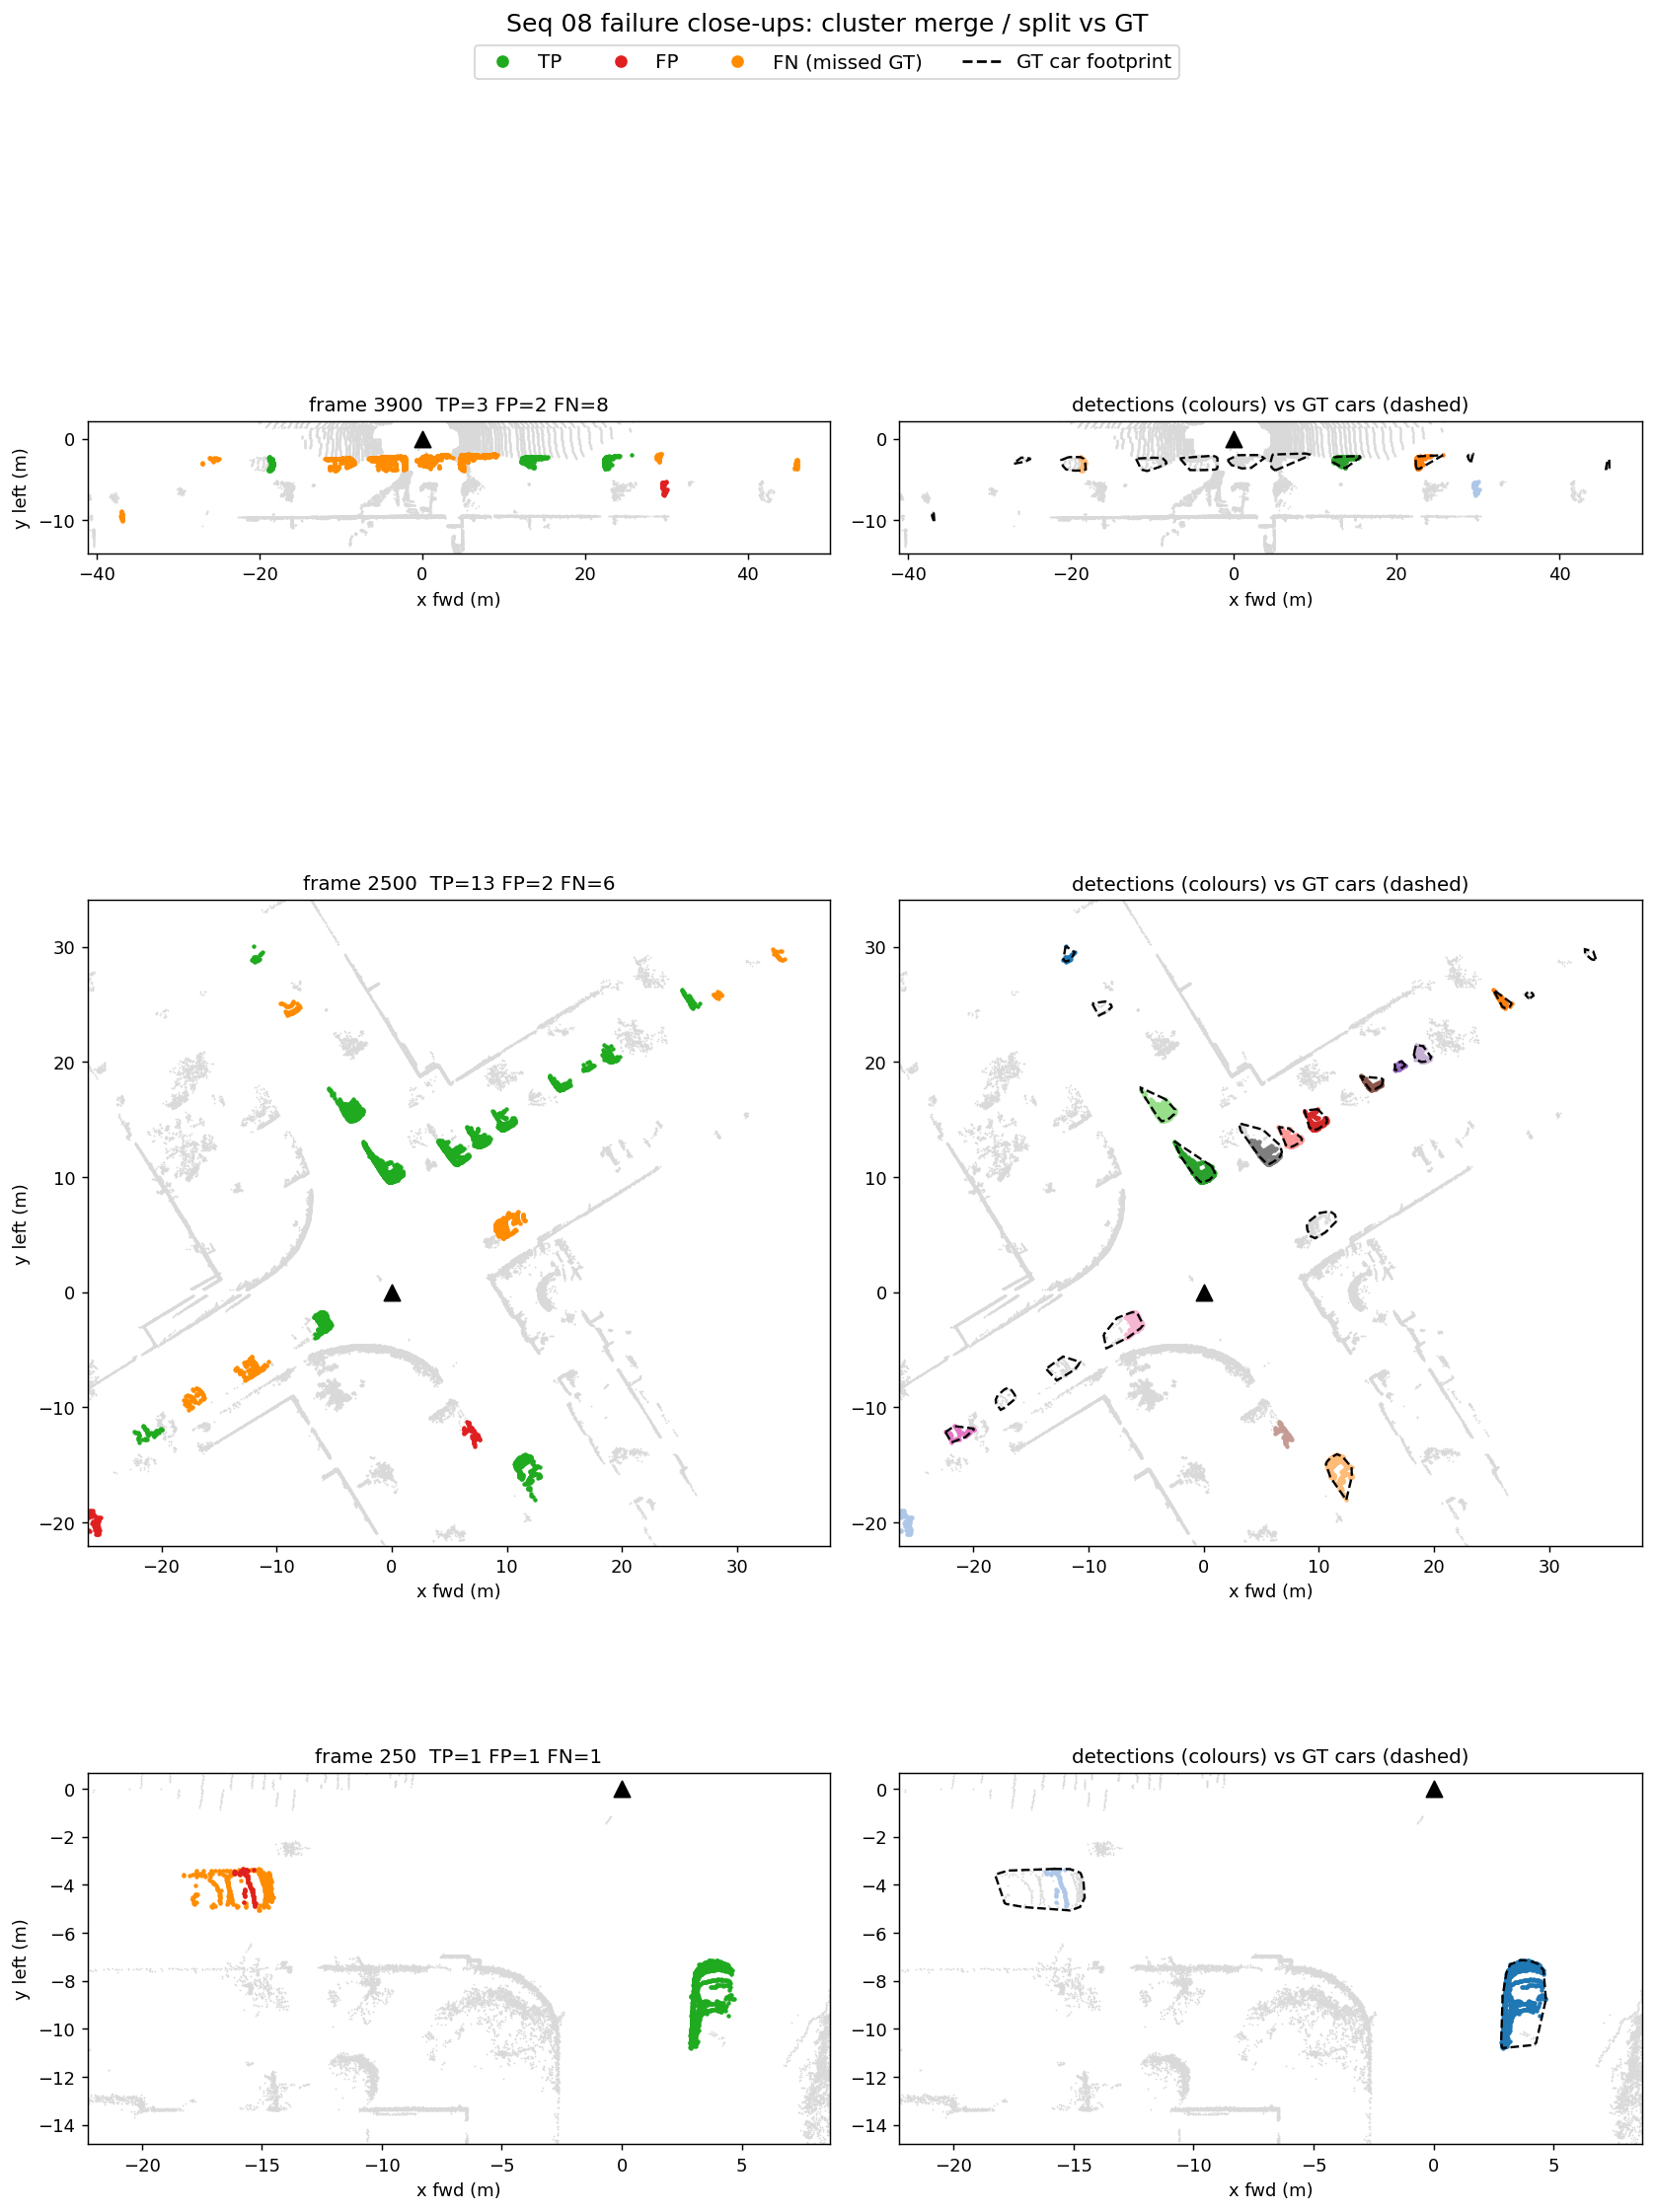
\includegraphics[width=\linewidth]{seq08_failure_zooms.png}
  \caption[Detection failure close-ups on seq~08]{Failure close-ups on sequence~08 (true positives green, false positives
    red, missed ground-truth cars orange; dashed outlines are ground-truth car
    footprints). Near-ego missed cars are fragmented into several small point groups
    rather than one cluster, matching the split mechanism of
    Table~\ref{tab:split}. Although the panel title mentions both merge and split,
    merging is measured at $\leq\!\SI{0.5}{\percent}$ (Table~\ref{tab:split}), so the
    misses shown are fragmentation, not fusion of neighbouring cars.}
  \label{fig:failure-zooms}
\end{figure}

\subsection{Limits of the Repair Strategies}
\label{sec:repairs}

Given that splitting caps recall, the obvious responses fall into two families:
change how clusters form (a larger minimum cluster size, a different
clusterer, distance-adaptive parameters, or pre-clustering point accumulation) or
reassemble fragments after HDBSCAN has split them. We tried six in total;
Table~\ref{tab:strategies} collects the four with a reproducible quantitative
outcome, and two further strategies (temporal accumulation and threshold lowering)
are discussed in prose below. All were evaluated against the same pre-promotion
sequence-00 baseline (full pipeline, classifier and track filter on;
$F_1=\num{0.844}$), and the load-bearing ones were re-checked on the held-out
sequence~08.

\begin{table}[H]
  \centering
  \caption[Recall-repair strategies]{Recall-repair strategies against the pre-promotion baseline (full
    pipeline, classifier and track filter on, on a sequence-00 sample; held-out
    sequence-08 $F_1$ where measured). This is an exploratory pre-promotion repair
    search: it predates the coarse-voxel configuration of
    Section~\ref{sec:resolution-fix} (which is why the baseline here is
    $F_1=\num{0.844}$, not the promoted headline), and it is reported to establish the
    mechanism by which each strategy fails rather than as headline metrics. Every
    strategy either loses $F_1$ outright or fails to hold its sequence-00 gain on the
    held-out sequence; the adopted resolution and its full-sequence numbers are given in
    Section~\ref{sec:resolution-fix}. Sources in the ``Src'' column are
    finding numbers. Two further strategies, temporal point accumulation and
    lowering the size thresholds, are discussed in the text but omitted here:
    temporal accumulation is single-sourced to a reverted feature in the session
    log (not reproducible under the research freeze), and threshold lowering
    produced no change in true positives; both belong in prose rather than the main
    results table.}
  \label{tab:strategies}
  \setlength{\tabcolsep}{4pt}
  \begin{tabular}{lcccc}
    \toprule
    Strategy & Seq 00 $P$ & Seq 00 $R$ & Seq 00 $F_1$ & Seq 08 $F_1$ \\
    \midrule
    Baseline (HDBSCAN, MCS \num{10}) & 0.984 & 0.739 & \textbf{0.844} & \textbf{0.829} \\
    BEV clustering (res \SI{0.30}{\metre})   & 0.993 & 0.640 & 0.779 &, \\
    Higher MCS \num{20}                       & 0.976 & 0.755 & 0.852 & 0.801 \\
    Fragment merge (\SI{1.5}{\metre}, \num{30}\,pt) & 0.931 & 0.755 & 0.834 & 0.815 \\
    Adaptive HDBSCAN (\num{30}/\num{15}/\num{10}) & 0.935 & 0.748 & 0.831 &, \\
    \bottomrule
  \end{tabular}
\end{table}

Each strategy fails for a structural reason, and the reasons are consistent with the
diagnosis of Section~\ref{sec:split-analysis}:

\begin{itemize}
  \item Higher minimum cluster size (MCS \num{20}) is the most instructive.
    It is the only variant to improve $F_1$ on sequence~00
    (\num{0.844}~$\rightarrow$~\num{0.852}), by discouraging the small splinter
    clusters. But it does not generalise: on the held-out sequence~08 it drops to
    $F_1$~\num{0.801}, below the \num{0.829} baseline, because a larger
    minimum also erases genuinely sparse distant cars. The sequence-00 gain was
    over-fitting.
  \item Post-clustering fragment merge (join clusters within
    \SI{1.5}{\metre}) raises sequence-00 recall to \num{0.755} but loses precision
    (\num{0.984}~$\rightarrow$~\num{0.931}), because the same proximity rule also
    fuses nearby non-car structure (walls, poles) into oversized clusters. On
    held-out data the precision loss cancels the recall gain
    ($F_1$~\num{0.815}~$<$~\num{0.829}).
  \item Distance-adaptive HDBSCAN (a larger minimum cluster size near the
    ego, smaller far away) introduces boundary artefacts at the ring transitions and
    is worse than the global setting.
  \item Bird's-eye-view clustering, a cheaper
    connected-component alternative, collapses recall to \num{0.640}: projecting to
    two dimensions merges objects that overlap in the ground plane but are separated
    in height, and morphological cleanup destroys sparse distant clusters.
  \item Temporal aggregation, accumulating object points over three
    consecutive frames before clustering, to densify sparse cars, collapses the
    pipeline ($F_1$~\num{0.073}, recall \num{0.039}).\footnote{Source:
    \texttt{docs/session\_history.md} (2026-06 exploratory session). The
    \texttt{temporal\_window} feature was implemented and then fully reverted, so
    this result is on the pre-promotion baseline and was not re-run under the
    research freeze; it is reported here in prose, not in Table~\ref{tab:strategies},
    for that reason, and its value is the mechanism below rather than the exact
    figure.} Accumulating points does not densify
    the existing clusters; it reshapes the clustering landscape entirely
    (about \num{134000} accumulated points yield \num{645}+ clusters versus
    $\sim$\num{240} single-frame, of which fewer pass the geometric filters,
    \num{17} versus \num{34}).
  \item Lowering the cluster-size thresholds to admit sparser groups
    produced no change in true positives at all: the binding constraint is cluster
    quality, not the count threshold, so relaxing the threshold merely admits more
    noise (\texttt{docs/session\_history.md}).
\end{itemize}

The failure modes are strategy-specific, over-fitting, precision loss, ring
artefacts, projection ambiguity, a reshaped clustering landscape, but they share
a limit. The two strategies that reassemble after the split (fragment merge, and to
a lesser extent the proximity-based part of the adaptive scheme) run into the fact
that density-based clustering has no notion of objectness: once a dense car is
partitioned along an internal density gap, no proximity- or size-based rule can
reliably tell ``rejoin these two fragments of one car'' apart from ``do not join
these two adjacent cars.'' The strategies that instead change how clusters
form, a larger minimum size, a different clusterer, per-ring parameters,
pre-clustering accumulation, avoid the reassembly trap but hit the same wall from
the other side: any single global density criterion that is loose enough to keep a
split car whole is also loose enough to fuse a close pair, so a sequence-00 gain
becomes a held-out loss. The one lever that helped, changing the clustering
resolution (Section~\ref{sec:resolution-fix}), is also a formation change; it
works not by escaping this limit but by happening to sit at a resolution that closes
intra-car gaps before it starts closing inter-car ones. This is why the earlier
project conclusion, that recall was fixed at a hard ceiling of about \num{0.74}
, was reasonable given only the evidence
in Table~\ref{tab:strategies}, and also, as the next section shows, wrong: it read a
limit on these repairs as a limit on the approach.

\subsection{Clustering Resolution and the Corrected Ceiling}
\label{sec:resolution-fix}

The intervention that helped was not a repair at all but a change to the clustering
resolution: re-voxelising the object cloud to a \SI{0.10}{\metre} grid
before running HDBSCAN, rather than clustering the full-resolution
\SI{0.05}{\metre} cloud (adopted in the runtime optimisation of
Section~\ref{sec:results-runtime}). A coarser grid closes the small intra-car density gaps that HDBSCAN was
cutting along, so fewer splits form in the first place. It is a formation change like
the failed ones in Section~\ref{sec:repairs}, but it lands on the favourable side of
the trade described there, coarse enough to close intra-car gaps, still fine
enough not to fuse neighbouring cars.

\begin{table}[H]
  \centering
  \caption[Effect of coarsening the clustering voxel]{Effect of coarsening the clustering voxel from \SI{0.05}{\metre} to
    \SI{0.10}{\metre} on the split rate (full sequence~08, \num{34057}
    ground-truth cars). Coarsening removes splits but is not free: it also
    fuses some neighbouring cars, so the merge count rises even as the split rate falls.}
  \label{tab:splitrate}
  \begin{tabular}{lcc}
    \toprule
    & Full-res (\SI{0.05}{\metre}) & Coarse (\SI{0.10}{\metre}) \\
    \midrule
    clustered ``ok''            & 18769 (55.1\%) & 22487 (66.0\%) \\
    split                        & 15245 (44.8\%) & 11480 (33.7\%) \\
    merged (cross-cutting)       & 56 (0.2\%)     & 284 (0.8\%)    \\
    mean clusters per split car  & 4.7            & 3.0 \\
    \bottomrule
  \end{tabular}
\end{table}

Table~\ref{tab:splitrate} shows the split rate falling by \num{11.1} points
(\SI{44.8}{\percent}~$\rightarrow$~\SI{33.7}{\percent}). This is a trade, not a
free lunch: the coarser grid also fuses some adjacent cars, so the merged count
rises from \num{56} to \num{284} (\SI{0.2}{\percent}~$\rightarrow$~\SI{0.8}{\percent}).
The gain still dominates, roughly \num{3700} cars move from split to clean while
about \num{230} newly merge, but the merge cost is real and bounds how far
coarsening can be pushed.
At the pipeline level, on the full sequence~08, this lifts recall from \num{0.710} to
\num{0.732} ($+\num{756}$ true positives) with precision essentially unchanged
(\num{0.910}~$\rightarrow$~\num{0.911}) and $F_1$ from \num{0.798} to \num{0.812}. The same coarsening also reduces clustering runtime, which is why it
was adopted; its detection benefit is the subject here and its runtime co-benefit is
reported in Section~\ref{sec:results-runtime}.

This result forces a correction to the earlier ceiling claim, which we state plainly
rather than bury. The ``$\sim$\num{0.74}
hard limit'' was partly a resolution artefact, not a fundamental property of
the approach: the strategies of Section~\ref{sec:repairs} genuinely do fail, but none
of them tried this particular resolution setting, and changing it recovered part of
the loss. The standing recommendation is therefore
\texttt{cluster\_voxel\_size}~$=\SI{0.10}{\metre}$ in production, not ``accept
\num{0.74}.''

A smaller structural limit does remain, and it is architectural. Coarsening the voxel
further would eventually start merging adjacent cars, trading the split problem for a
merge problem; and the clustering-method benchmark of Section~\ref{sec:results-ablations}
shows that no fixed-radius density clusterer, at any tested radius, reaches even
HDBSCAN's recall. The ceiling that remains is the one imposed by density-based
clustering having no model of what a car is: it groups points by proximity and
density alone, so it cannot be pushed to the recall of a learned object detector by
tuning. Reaching that level would require replacing the clustering stage with a
learned detector, which is outside the scope of this thesis (Chapter~\ref{ch:conclusion}). The
value of this analysis is to have located the ceiling precisely, it is in
the clustering stage, it is splitting rather than classification or merging, and it
is lower than first claimed, and to have mapped which repairs cannot move it and
which one can.

\subsection{Recall Analysis: Summary}
\label{sec:recall-summary}

The recall shortfall is clustering-bound, not classifier-bound: the classifier and
track filter sit on top of a recall ceiling that geometric clustering already imposes
(Section~\ref{sec:recall-diagnosis}). The dominant mechanism is HDBSCAN splitting
large, close cars into fragments, \SI{33.7}{\percent} of cars at the adopted resolution, worst at
short range, while merging is negligible, and the cleanly-clustered fraction sits
just below the achieved recall, so most split cars are lost
(Section~\ref{sec:split-analysis}). A search of six repair strategies, higher
minimum cluster size, fragment merging, adaptive and BEV clustering, temporal
accumulation, and threshold lowering, all fail to generalise, for a shared reason:
density-based clustering has no notion of objectness, so any criterion loose enough to
keep a split car whole also fuses adjacent cars, and reassembling fragments after the
split faces the same ambiguity (Section~\ref{sec:repairs}). The one effective lever was clustering
resolution: a coarser pre-clustering voxel prevents splits from forming, lifting
recall \num{0.710}~$\rightarrow$~\num{0.732} and correcting the earlier overstated
``hard ceiling'' (Section~\ref{sec:resolution-fix}). The residual limit is
architectural, density clustering has no notion of objectness, and is carried
to the limitations and future-work discussion of Chapter~\ref{ch:conclusion}.



% Chapter-summary section removed to mirror the gospel's lean Ch.4; its results
% recap and limitations are carried in Chapter~\ref{ch:conclusion} (Established
% Results and Their Reach; Limitations and Discussion).
